\documentclass{article}
\usepackage[utf8]{inputenc}
\usepackage{geometry}
\usepackage{graphicx}
\usepackage{amsmath}
\usepackage{amsfonts}
\usepackage{amsthm}
\usepackage{amssymb}
\usepackage[most]{tcolorbox}
\usepackage{array}
\usepackage{latexsym}
\usepackage{alltt}
\usepackage{hyperref}
\usepackage{color, colortbl}
\usepackage{float}
\usepackage{pdfpages}
\usepackage{algpseudocode}
\usepackage{multicol}
\usepackage{multirow}
\usepackage{caption}
\usepackage{xparse}
\usepackage{setspace}
\usepackage{enumitem}
\usepackage{pdflscape}
% \usepackage{parskip}
\usepackage{blindtext}
\usepackage{forest}
\usepackage[newfloat]{minted}
\usepackage{booktabs}


\geometry
{
  a4paper,
  left=12mm,
  right=12mm,
  top=12mm,
  bottom=15mm,
}

% mybox
\newtcolorbox{mybox}[3][]
{
  colframe = #2!25,
  colback  = #2!10,
  coltitle = #2!20!black,  
  title    = {#3},
  #1,
}

\definecolor{ex}{rgb}{1.00,0.65,0.00}
\definecolor{bg}{rgb}{0.95,0.95,0.95}
\setminted
{
	mathescape=true,
	xleftmargin=\parindent,
	bgcolor=bg,
	escapeinside=@@
}

\SetupFloatingEnvironment{listing}{name=Code}

% New environments that use mybox
\newcounter{example}%[section]
\newenvironment{example}[1]{\begin{mybox}[breakable]{ex}{\refstepcounter{example}\textbf{Example \theexample #1}}}{\end{mybox}}

\newcounter{definition}%[section]
\newenvironment{definition}[1]{\refstepcounter{definition}\begin{mybox}[breakable]{blue}{\textbf{Definition \thedefinition #1}}}{\end{mybox}}

\newcounter{theorem}%[section]
\newenvironment{theorem}[1]{\begin{mybox}{red}{\refstepcounter{theorem}\textbf{Theorem \thetheorem #1}}}{\end{mybox}}

\newenvironment{formula}[1]{\begin{mybox}{cyan}{\textbf{#1}}}{\end{mybox}}

% Changing maketitle
\makeatletter         
\renewcommand\maketitle{
{\raggedright % Note the extra {
\begin{center}
{\Large \bfseries \@title}\\[2ex] 
{\large \@author \ - \@date}\\[2ex]
\end{center}}} % Note the extra }
\makeatother

% \onehalfspacing % adjust spacing
\setlength{\parskip}{0.5\baselineskip}

% macros
\newcommand{\prob}[1]{\textbf{\textit{P}}\left\{#1\right\}}
\newcommand{\expc}[1]{\mathbf{E}\left(#1\right)}
\newcommand{\expcs}[1]{\mathbf{E}^2\left(#1\right)}
\newcommand{\expck}[2]{\mathbf{E}\left(#1^{#2}\right)}
\newcommand{\var}[1]{\text{Var}\left( #1 \right)}
\newcommand{\ra}{\rightarrow}
\newcommand{\la}{\leftarrow}
\newcommand{\tar}{\vartriangleright}
\newcommand{\Ra}{\Rightarrow}
\newcommand{\blank}{\sqcup}
\newcommand{\R}[2]{\tikz [remember picture,overlay] \node (#1) {#2};}
\newcommand{\bs}[1]{\boldsymbol{#1}}

\def\circtxt#1{$\mathalpha \bigcirc \mkern-13mu \mathtt #1$}
\def\smiley{\textcircled{\scriptsize $\mkern3mu\ddot{\ } \mkern-15mu \smallsmile$}}

\NewDocumentCommand{\dsum}{%
    e{^_}
}{%
  {% 
    \displaystyle\sum
    \IfValueT{#1}{^{#1}}
    \IfValueT{#2}{_{#2}}
  }
}%

% maketitle variables
\title{CENG 222 - Chapter 9: Statistical Inference I}
\author{Burak Metehan Tunçel}
\date{June 2022}

\begin{document}

\maketitle

\begin{multicols}{2}
\setlength{\columnsep}{1.5cm}
\setlength{\columnseprule}{0.2pt}

\section{Parameter Estimation}
\label{sec:parameter-estimation}

We have learned a few elementary ways to determine the \textit{family of distributions}. Now, we learn how to \textit{estimate parameters of distributions}. As a result, a large family will be reduced to just one distribution that we can use for performance evaluation, forecasting, etc.

Statisticians developed a number of estimation techniques, each having certain optimal properties. Two rather popular methods are discussed in this section:
\begin{itemize}
  \item method of moments, and
  \item method of maximum likelihood.
\end{itemize}

\subsection{Method of Moments}
\label{subsec:method-of-moments}

\subsubsection{Moments}
\label{subsubsec:moments}

First, let us define the moments.
\begin{definition}{}
  The $k$-th \textbf{population moment} is defined as
  \begin{equation*}
    \mu_k = \expck{X}{k}
  \end{equation*}
  The $k$-th \textbf{sample moment}
  \begin{equation*}
    m_k = \frac{1}{n} \sum_{i=1}^{n} X_i^k
  \end{equation*}
  estimates $\mu_k$ from a sample $(X_1,\ \ldots,\ X_n)$. \\

  The first sample moment is the sample mean $\bar{X}$.  
\end{definition}

Central moments are computed similarly, after centralizing the data, that is, subtracting the mean.

\begin{definition}{}
  For $k \geq 2$, the $k$-th \textbf{population central moment} is defined as
  \begin{equation*}
    \mu_k' = \expck{(X - \mu_1)}{k}
  \end{equation*}
  The $k$-th \textbf{sample central moment}
  \begin{equation*}
    m_k' = \frac{1}{n} \sum_{i=1}^{n} (X_i - \bar{X})^k
  \end{equation*}
  estimates $\mu_k$ from a sample $(X_1,\ \ldots,\ X_n)$.
\end{definition}

\textbf{Remark:} 
\begin{itemize}
  \item The \textit{second population central moment is variance} $\var{X}$.
  \item The \textit{second sample central moment is sample variance}, although $(n - 1)$ in its denominator is now replaced by $n$.
\end{itemize}
We mentioned that estimation methods are not unique. For unbiased estimation of $\sigma^2 = \var{X}$, we use
\begin{equation*}
  s^2 = \frac{1}{n - 1} \sum_{i=1}^{n} (X_i - \bar{X})^2
\end{equation*}
however, method of moments and method of maximum likelihood produce a different version,
\begin{equation*}
  S^2 = m_2' = \frac{1}{n} \sum_{i=1}^{n} (X_i - \bar{X})^2
\end{equation*}


\subsubsection{Estimation}
\label{subsubsec:estimation}

\textbf{Method of moments} is based on a simple idea. Since our sample comes from a family of distributions $\{ F(\theta) \}$, we choose such a member of this family whose properties are close to properties of our data. Namely, we shall \textit{match the moments}.

To estimate $k$ parameters, equate the first $k$ population and sample moments,
\begin{equation*}
  \begin{cases}
    \mu_1 = m_1 \\
    \cdots\ \cdots\ \cdots \\
    \mu_k = m_k \\
  \end{cases}
\end{equation*}
The left-hand sides of these equations depend on the distribution parameters. The right-hand sides can be computed from data. The \textbf{method of moments estimator} is the solution of this system of equation.

\begin{example}{ (Poisson)}
  To estimate parameter $\lambda$ of Poisson($\lambda$) distribution, we recall that
  \begin{equation*}
    \mu_1 = \expc{X} = \lambda
  \end{equation*}
  There is only one unknown parameter, hence we write one equation,
  \begin{equation*}
    \mu_1 = \lambda = m_1 = \bar{X}
  \end{equation*}
  ``Solving'' it for $\lambda$, we obtain
  \begin{equation*}
    \hat{\lambda} = \bar{X}
  \end{equation*}
  the method of moments estimator of $\lambda$.
\end{example}

\textbf{\textit{Check the examples 9.4 and 9.5 from textbook.}}

\noindent On rare occasions, when $k$ equations are not enough to estimate $k$ parameters, we'll consider higher moments.

\vspace*{\fill}
\columnbreak

\begin{example}{ (Normal)}
  Suppose we already know the mean $\mu$ of a Normal distribution and would like to estimate the variance $\sigma^2$. Only one parameter $\sigma^2$ is unknown; however, the first method of moments equation
  \begin{equation*}
    \mu_1 = m_1
  \end{equation*}
  does not contain $\sigma^2$ and therefore does not produce its estimate. We then consider the second equation, say,
  \begin{equation*}
    \mu_2' = \sigma^2 = m_2' = S^2
  \end{equation*}
  which gives us the method of moments estimate immediately, $\hat{\sigma}^2 = S^2$.
\end{example}

Method of moments estimates are typically easy to compute. They can serve as a quick tool for estimating parameters of interest.


\subsection{Method of Maximum Likelihood}
\label{subsec:method-of-maximum-likelihood}

Since the sample $\boldsymbol{X} = (X_1,\ \ldots,\ X_n)$ has already been observed, we find such parameters that maximize the probability (likelihood) for this to happen. In other words, we make the event that has already happened to be as likely as possible. This is yet another way to make the chosen distribution consistent with the observed data.
\begin{definition}{}
  \textbf{Maximum likelihood estimator} is the parameter value that maximizes the likelihood of the observed sample.
  \begin{itemize}
    \item For a discrete distribution, we maximize the joint pmf of data $P(X_1,\ \ldots,\ X_n)$.
    \item For a continuous distribution, we maximize the joint density $f(X_1,\ \ldots,\ X_n)$.
  \end{itemize}
\end{definition}

\subsubsection{Discrete Case}
\label{subsubsec:disc-case}

For a discrete distribution, the probability of a given sample is the joint pmf of data,
\begin{align*}
  \prob{\boldsymbol{X} = (X_1,\ \ldots,\ X_n)} = P(\boldsymbol{X}) &= P(X_1,\ \ldots,\ X_n) \\
  &= \prod_{i=1}^{n} P(X_i)
\end{align*}
because in a simple random sample, all observed $X_i$ are independent.

To maximize this likelihood, we consider the critical points by taking derivatives with respect to all unknown parameters and equating them to 0.  The maximum can only be attained at such parameter values $\theta$ where the derivative $\frac{\partial}{\partial\theta} P(X)$ equals 0, where it does not exist, or at the boundary of the set of possible values of $\theta$.

A nice computational shortcut is to take logarithms first. Differentiating the sum
\begin{equation*}
  \ln \prod_{i=1}^{n} P(X_i) = \sum_{i=1}^{n} \ln P(X_i)
\end{equation*}
is easier than differentiating the product $\prod P(X_i)$. Besides, logarithm is an increasing function, so the likelihood $P(\boldsymbol{X})$ and the log-likelihood $\ln P(\boldsymbol{X})$ are maximized by exactly the same parameters.

\textbf{\textit{Check the example 9.7 from textbook.}}

\subsubsection{Continuous Case}
\label{subsubsec:cont-case}

In the continuous case, the probability to observe exactly the given number $X = x$ is $0$. Instead, the method of maximum likelihood will maximize the
probability of observing ``almost'' the same number.

For a very small $h$,
\begin{equation*}
  \prob{x - h < X < x + h} = \int_{x - h}^{x + h} f(y) d(y) \approx (2h) f(x)
\end{equation*}
That is, the probability of observing a value close to $x$ is proportional to the density $f(x)$ (see Figure 1). Then, for a sample $\bs{X} = (X_1,\ \ldots,\ X_n)$, the maximum likelihood method will maximize the joint density $f(X_1,\ \ldots,\ X_n)$.
\begin{figure}[H]
  \centering
  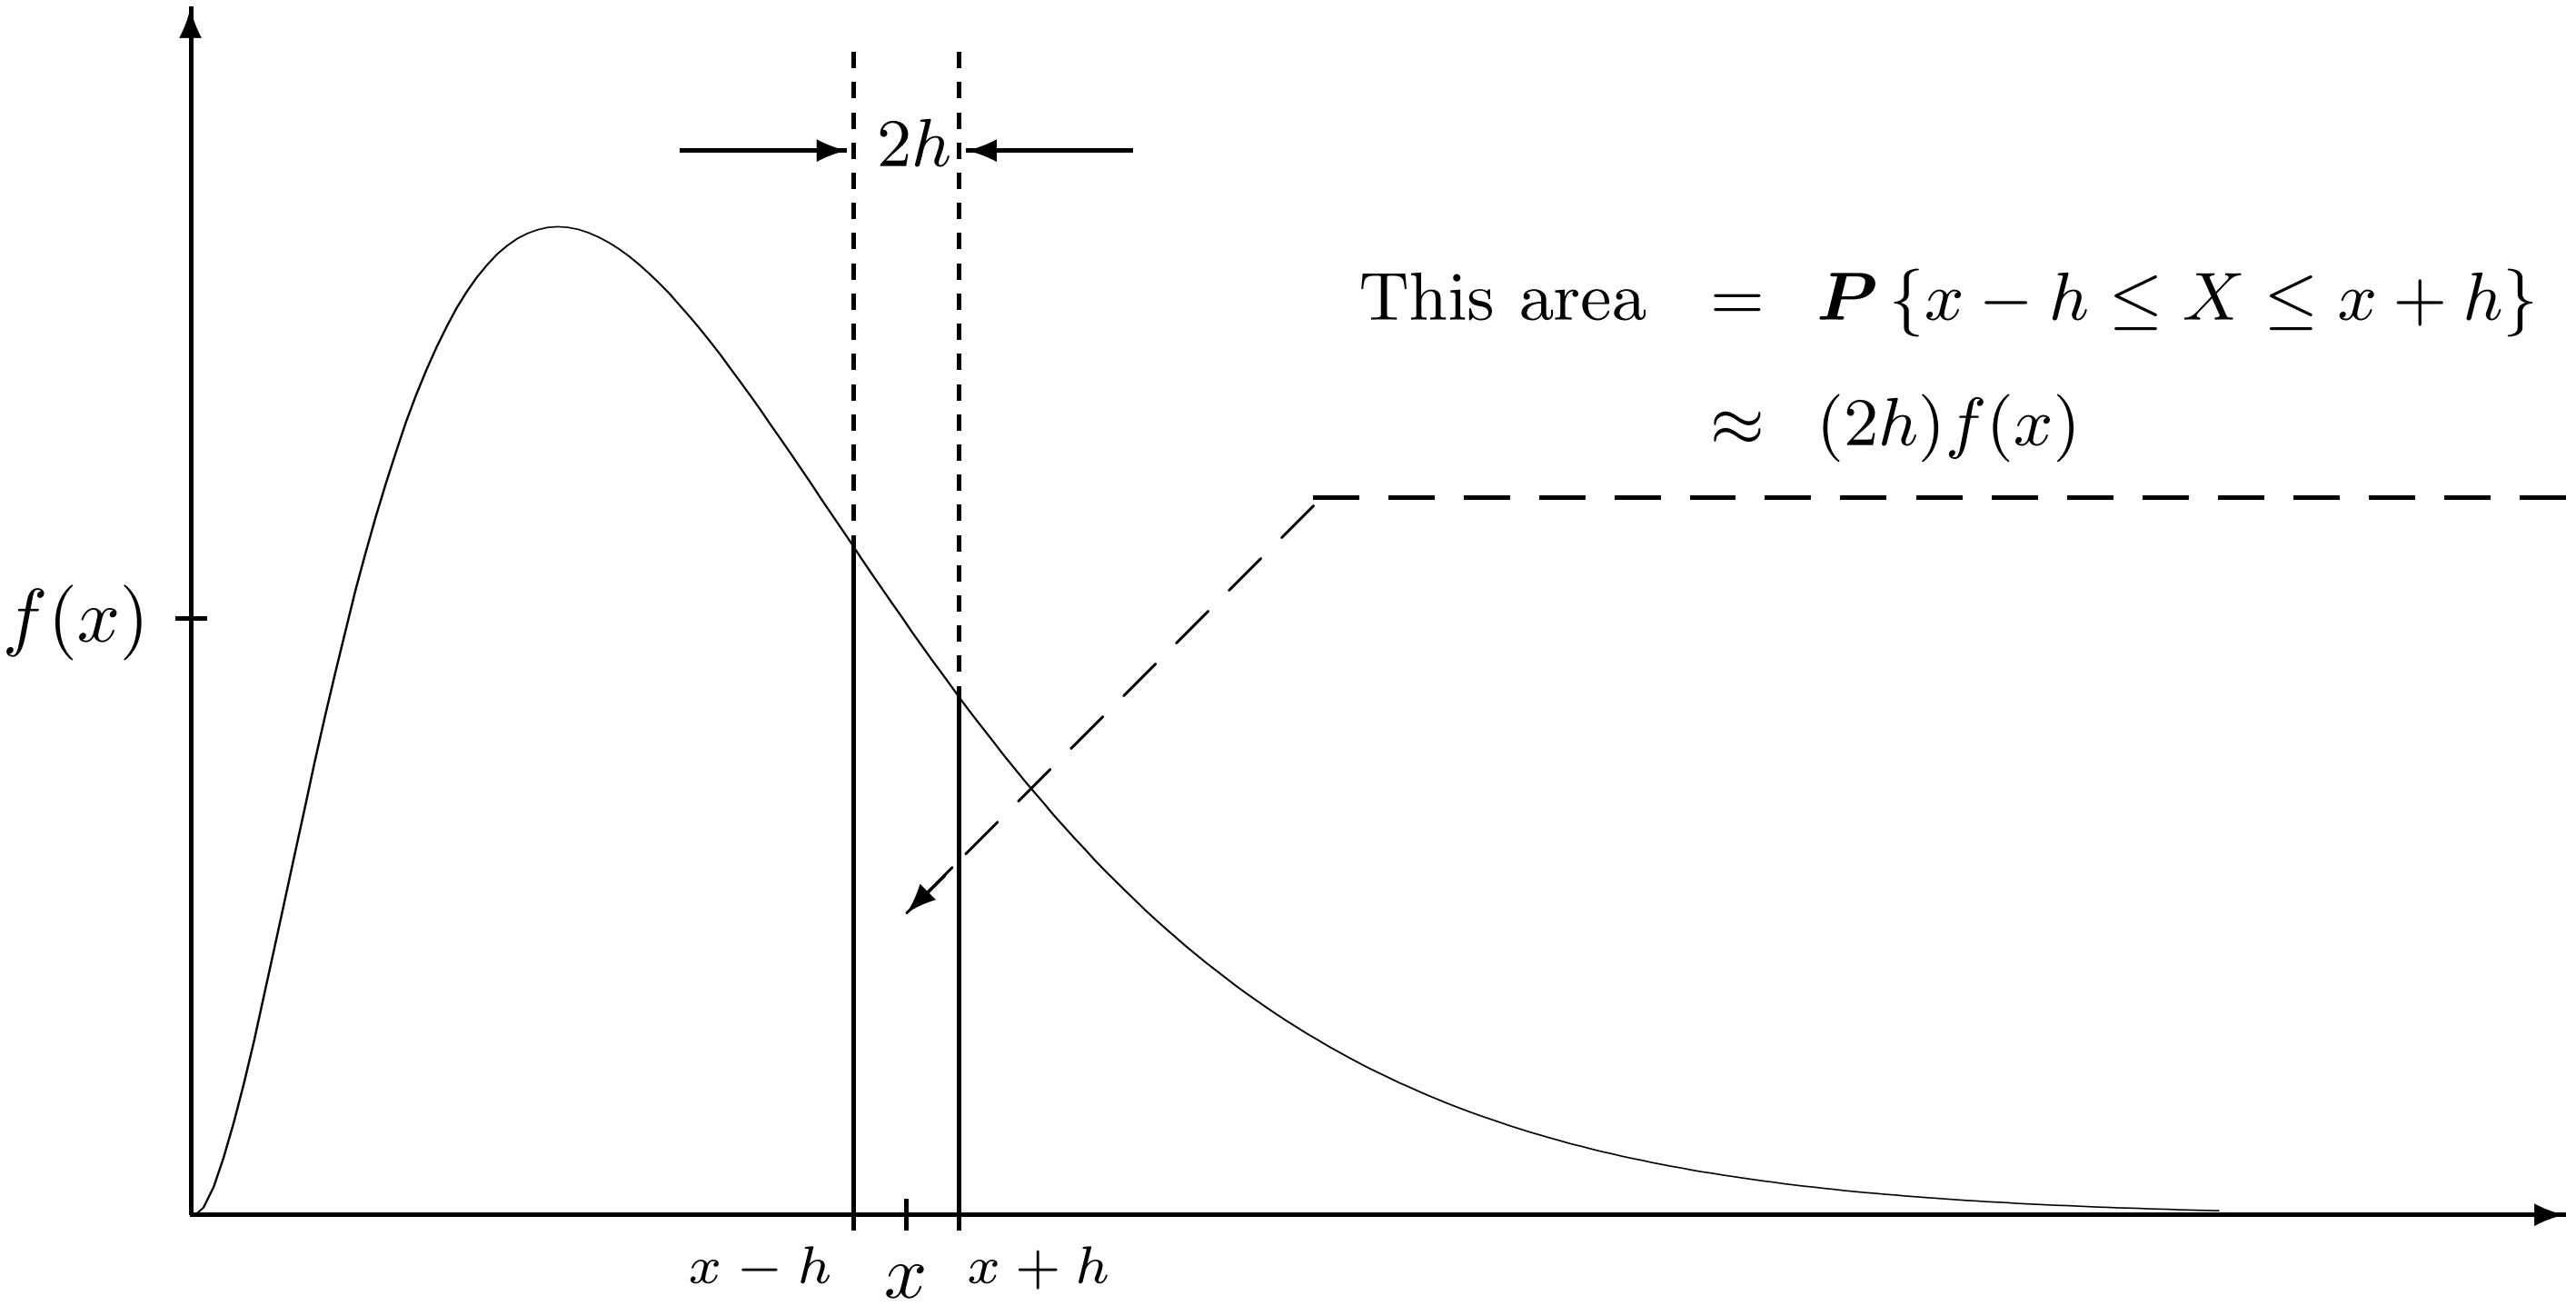
\includegraphics[width=\linewidth]{img/fig-9.1.png}
  \caption{}
  \label{fig:9.1}
\end{figure}

\textbf{\textit{Check the examples 9.8 and 9.9 from textbook.}}

Sometimes the likelihood has no critical points inside its domain, then it is maximized at the boundary.

When we estimate more than $1$ parameter, all the partial derivatives should be equal $0$ at the critical point. If no critical points exist, the likelihood is again maximized on the boundary.

Maximum likelihood estimators are rather popular because of their nice properties. Under mild conditions, these estimators are consistent, and for large samples, they have an approximately Normal distribution. Often in complicated problems, finding a good estimation scheme may be challenging whereas the maximum likelihood method always gives a reasonable solution.

\vspace*{\fill}
\columnbreak


\subsection{Estimation of Standard Errors}
\label{subsec:estimation-of-standard-errors}

Standard errors can serve as measures of their accuracy. To estimate them, we derive an expression for the standard error and estimate all the unknown parameters in it.

\begin{example}{ (Estimation of the Poisson Parameter)}
  By the method of moments and maximum likelihood estimators of the Poisson parameter $\lambda$ is $\hat{\lambda} = \bar{X}$. Let us now estimate the
  standard error of $\hat{\lambda}$.

  \textbf{Solution:}
  There are at least two ways to do it.

  On one hand, $\sigma = \sqrt{\lambda}$ for the Poisson($\lambda$) distribution, so $\sigma(\hat{\lambda}) = \sigma(\bar{X}) = \sigma / \sqrt{n} = \sqrt{\lambda / n}$, as we know before (\textit{textbook (8.2) on p. 213}). Estimating $\lambda$ by $\bar{X}$, we obtain
  \begin{equation*}
    s_1(\hat{\lambda}) = \sqrt{\frac{\bar{X}}{n}} = \frac{\sqrt{\Sigma X_i}}{n}
  \end{equation*}

  On the other hand, we can use the sample standard deviation and estimate the standard error of the sample mean,
  \begin{equation*}
    s_2(\hat{\lambda}) = \frac{s}{\sqrt{n}} = \sqrt{\frac{\Sigma (X_i - \bar{X})^2}{n (n-1)}}
  \end{equation*}
  Apparently, we can estimate the standard error of $\hat{\lambda}$ by two good estimators, $s_1$ and $s_2$.
\end{example}



\section{Confidence Intervals}
\label{sec:confidence-intervals}

When we report an estimator $\hat{\theta}$ of a population parameter $\theta$, we know that most likely
\begin{equation*}
  \hat{\theta} \neq \theta
\end{equation*}
due to a sampling error. We realize that we have estimated $\theta$ up to \textit{some error}.

Then how much can we trust the reported estimator? How far can it be from the actual parameter of interest? What is the probability that it will be reasonably close? And if we observed an estimator $\hat{\theta}$, then what can the actual parameter $\theta$ be?

To answer these questions, statisticians use \textbf{confidence intervals}, which contain parameter values that deserve some confidence, given the observed data.
\begin{definition}{}
  An interval $\left[ a,\ b \right]$ is a $(1 - \alpha)100\%$ \textbf{confidence interval} for the parameter $\theta$ if it contains the parameter with probability $(1 - \alpha)$,
  \begin{equation*}
    \prob{a \leq \theta \leq b} = 1 - \alpha
  \end{equation*}
  The \textbf{coverage probability} $(1 - \alpha)$ is also called a \textbf{confidence level}.
\end{definition}

Let us take a moment to think about this definition. The probability of a random event $\{ a \leq \theta \leq b \}$ has to be $(1 - \alpha)$. What randomness is involved in this event?

The population parameter $\theta$ is not random. It is a \textit{population feature, independent of any random sampling procedure}, and therefore, it remains constant. On the other hand, the interval is computed from random data, and therefore, it is random. The coverage probability refers to the chance that our interval covers a constant parameter $\theta$.

\begin{figure}[H]
  \centering
  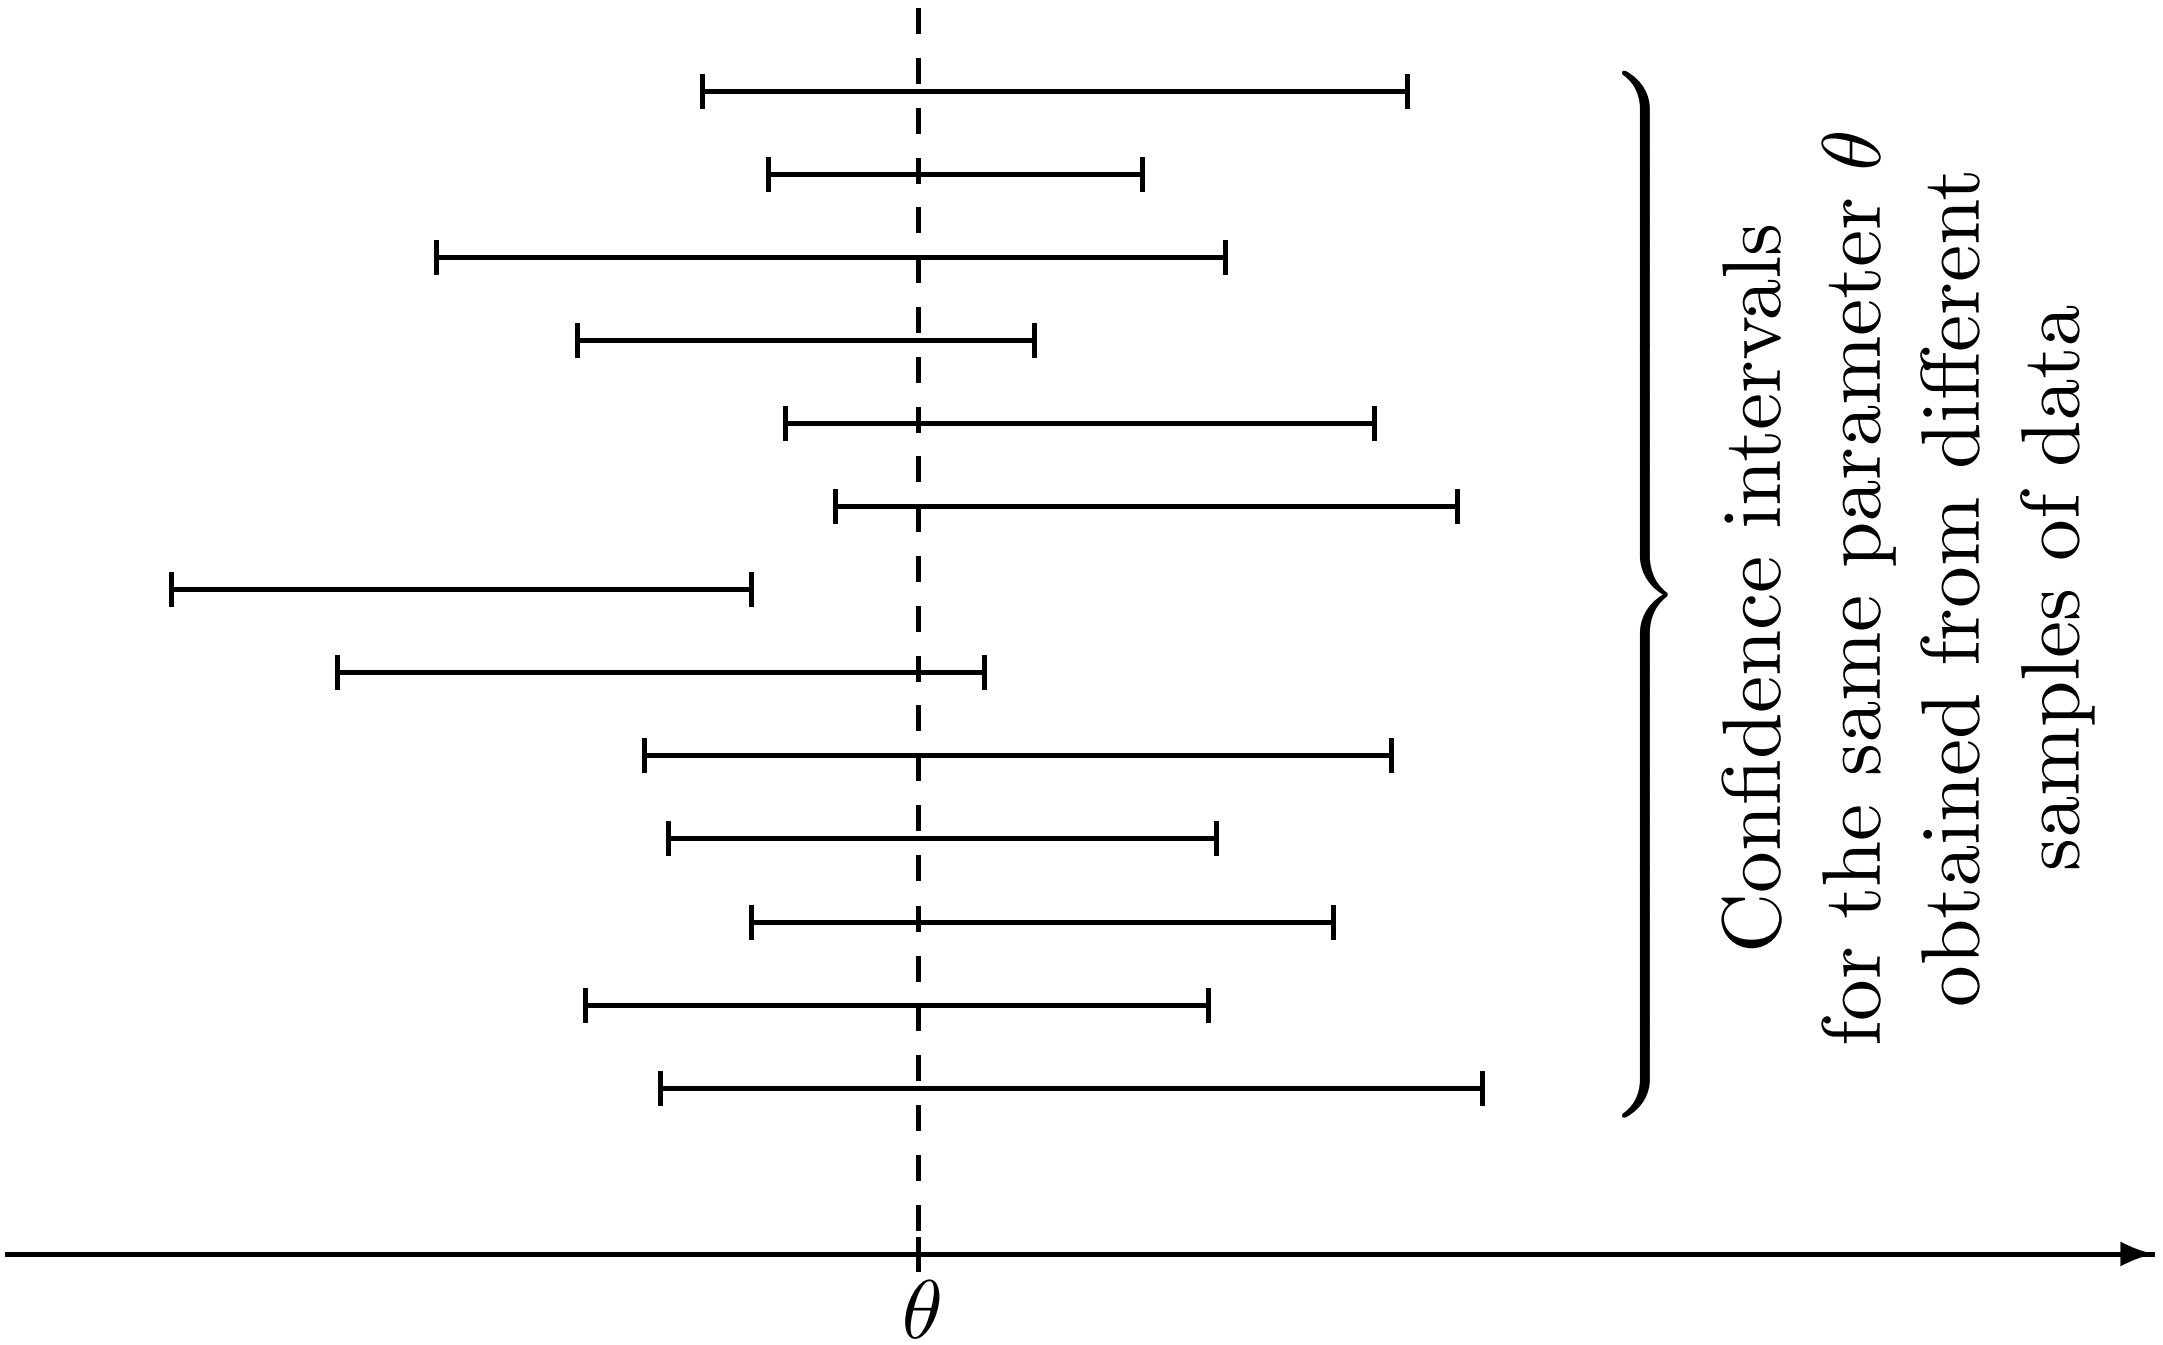
\includegraphics[width=\linewidth]{img/fig-9.2.png}
  \caption{}
  \label{fig:9.2}
\end{figure}

This is illustrated in Figure 2. Suppose that we collect many random samples and produce a confidence interval from each of them. If these are $(1 - \alpha)100\%$ confidence intervals, then we expect $(1 - \alpha)100\%$ of them to cover $\theta$ and $100\alpha\%$ of them to miss it. In Figure 2, we see one interval that does not cover $\theta$. No mistake was made in data collection and construction of this interval. It missed the parameter only due to a \textit{sampling error}.

It is therefore wrong to say, ``I computed a $90\%$ confidence interval, it is $\left[ 3,\ 6 \right]$. Parameter belongs to this interval with probability $90\%$''. The parameter is constant; it either belongs to the interval $\left[ 3,\ 6 \right]$ (with probability $1$) or does not. In this case, $90\%$ refers to the proportion of confidence intervals that contain the unknown parameter in a long run.

\subsection{Construction of Confidence Intervals: A General Method}
\label{subsec:const-of-conf-inter-a-gen-method}

Given a sample of data and a desired confidence level $(1 - \alpha)$, how can we construct a confidence interval $\left[ a,\ b \right]$ that will satisfy the coverage condition
\begin{equation*}
  \prob{a \leq \theta \leq b} = 1 - \alpha
\end{equation*}
in definition 4.

We start by estimating parameter $\theta$. Assume there is an unbiased estimator $\hat{\theta}$ that has a Normal distribution. When we standardize it, we get a Standard Normal variable
\begin{equation*}
  Z = \frac{\hat{\theta} - \mathbf{E}(\hat{\theta})}{\sigma(\hat{\theta})} = \frac{\hat{\theta} - \theta}{\sigma(\hat{\theta})}
\end{equation*}
where $\mathbf{E}(\hat{\theta}) = \theta$ because $\hat{\theta}$ is unbiased, and $\sigma(\hat{\theta}) = \sigma(\hat{\theta})$ is its standard error.

\vspace*{\fill}
\columnbreak

This variable falls between the Standard Normal quantiles $q_{\alpha/2}$ and $q_{1 - \alpha/2}$, denoted by
\begin{align*}
  - z_{\alpha/2} &= q_{\alpha / 2}\\
  z_{\alpha/2} &= q_{1 - \alpha / 2}\\
\end{align*}
with probability $(1 - \alpha)$, see Figure 3.
\begin{figure}[H]
  \centering
  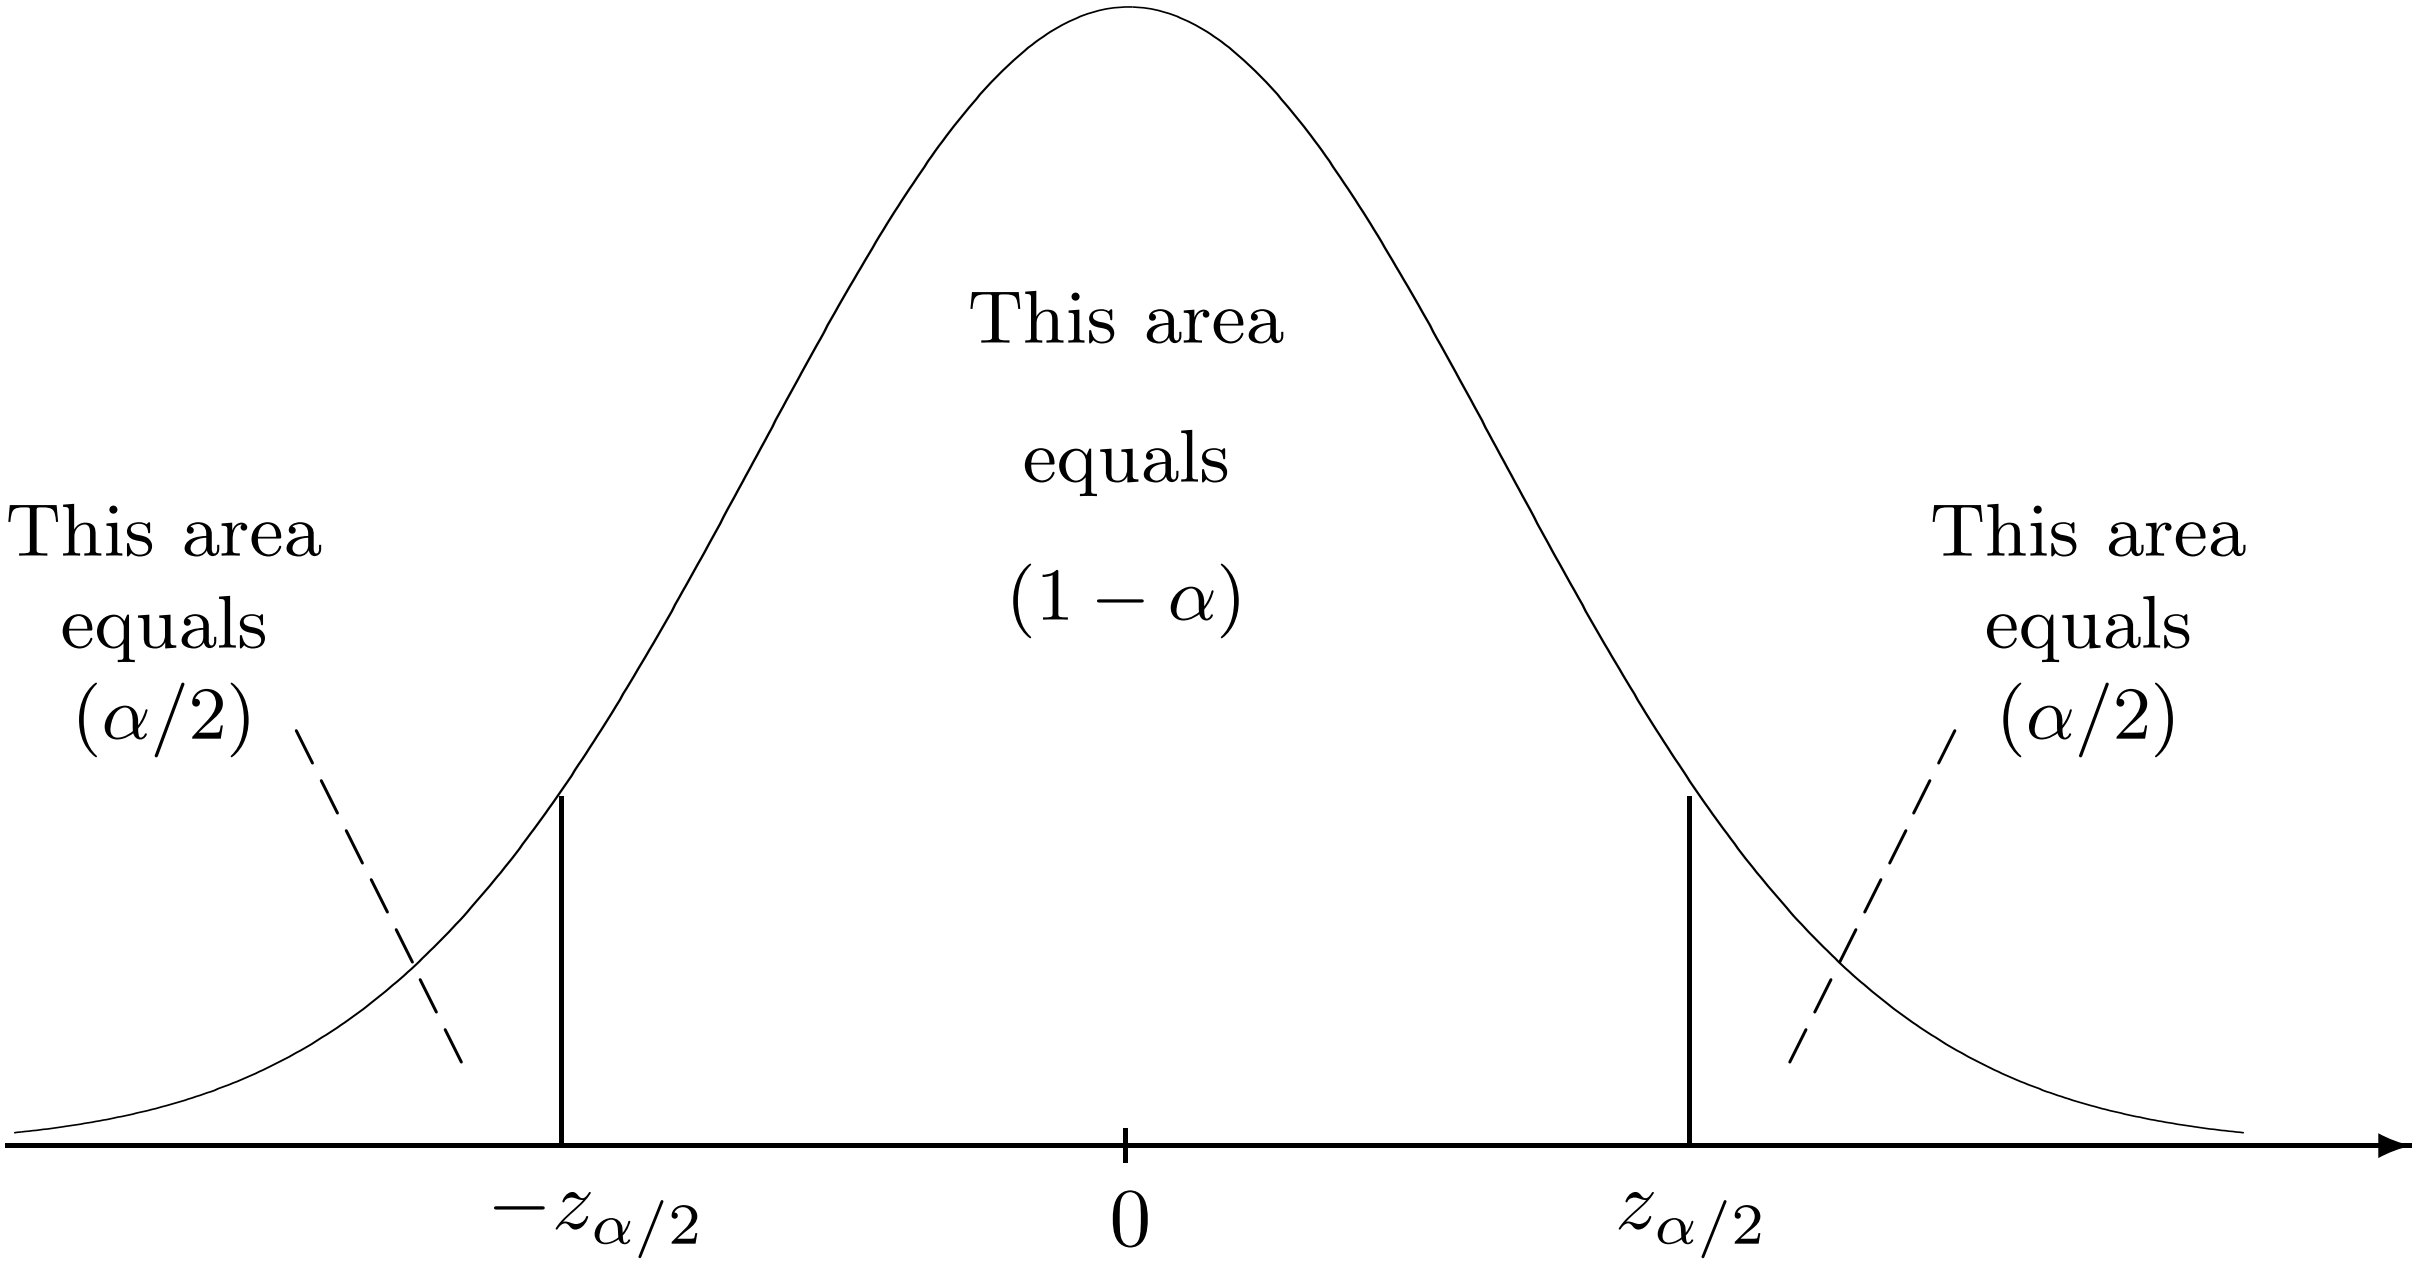
\includegraphics[width=\linewidth]{img/fig-9.3.png}
  \caption{}
  \label{fig:9.3}
\end{figure}

\noindent Then,
\begin{equation*}
  \prob{- z_{\alpha/2} \leq \frac{\hat{\theta} - \theta}{\sigma(\hat{\theta})} \leq z_{\alpha/2}} = 1 - \alpha
\end{equation*}
\noindent Solving the inequality inside $\{ \ldots \}$ for $\theta$, we get
\begin{equation*}
  \prob{
    \hat{\theta} - z_{\alpha/2} \cdot \sigma(\hat{\theta})
    \leq 
    \theta
    \leq
    \hat{\theta} + z_{\alpha/2} \cdot \sigma(\hat{\theta})
  } = 1 - \alpha
\end{equation*}
\noindent The problem is solved! We have obtained two numbers
\begin{align*}
  a &= \hat{\theta} - z_{\alpha/2} \cdot \sigma(\hat{\theta})\\
  b &= \hat{\theta} + z_{\alpha/2} \cdot \sigma(\hat{\theta})
\end{align*}
\noindent such that
\begin{equation*}
  \prob{a \leq \theta \leq b} = 1 - \alpha
\end{equation*}

\begin{formula}{Confidence interval, Normal distribution, Eq. 3}
  If parameter $\theta$ has an unbiased, Normally distributed estimator $\hat{\theta}$, then
  \begin{equation*}
    \hat{\theta} \pm z_{\alpha/2} \cdot \sigma(\hat{\theta}) = \left[ \hat{\theta} - z_{\alpha/2} \cdot \sigma(\hat{\theta}), \hat{\theta} + z_{\alpha/2} \cdot \sigma(\hat{\theta}) \right]
  \end{equation*}
  is a $(1 - \alpha)100\%$ confidence interval for $\theta$.

  If the distribution of $\hat{\theta}$ is \textit{approximately} Normal, we get an approximately $(1 - \alpha)100\%$ confidence interval.
\end{formula}

\setcounter{equation}{4}

In this formula, $\hat{\theta}$ is the \textbf{center of the interval}, and $z_{\alpha/2} \cdot \sigma(\hat{\theta})$ is the \textbf{margin}. The margin of error is often reported along with poll and survey results. In newspapers and press releases, it is usually computed for a $95\%$ confidence interval.

\begin{formula}{NOTATION}
  \begin{equation*}
    z_{\alpha} = q_{1 - \alpha} = \Phi^{-1} (1 - \alpha)
  \end{equation*}
  is the value of a Standard Normal variable $Z$ that is exceeded with probability $\alpha$
\end{formula}

\noindent Several important applications of this general method are discussed below. In each problem, we
\begin{enumerate}
  \item Find an unbiased estimator of $\theta$,
  \item Check if it has a Normal distribution,
  \item Find its standard error $\sigma(\hat{\theta}) = \textnormal{Std}(\hat{\theta})$,
  \item Obtain quantiles $\pm z_{\alpha/2}$ from the table of Normal distribution (Table A4 in the Appendix in textbook), and finally,
  \item Apply the rule (3).
\end{enumerate}

\subsection{Confidence Interval for the Population Mean}
\label{subsec:conf-inter-for-the-pop-mean}

Let us construct a confidence interval for the population mean
\begin{equation*}
  \theta = \mu = \expc{X}
\end{equation*}
\noindent Start with an estimator
\begin{equation*}
  \hat{\theta} = \bar{X} = \frac{1}{n} \sum_{i=1}^{n} X_i
\end{equation*}
\noindent The rule (3) is applicable in two cases.
\begin{enumerate}
  \item If a sample $\bs{X} = (X_1,\ \ldots,\ X_n)$ comes from Normal distribution, then $\hat{X}$ is also Normal, and rule (3) can be applied.
  \item If a sample comes from any distribution, but the sample size $n$ is large, then  $\hat{X}$ has an approximately Normal distribution according to the Central Limit Theorem. Then rule (3) gives an approximately $(1 - \alpha)100\%$ confidence interval.  
\end{enumerate}

The followings can be derived
\begin{align*}
  \expc{X} &= \mu &(\textnormal{unbiased estimator})\\
  \sigma(\bar{X}) &= \sigma / \sqrt{n}
\end{align*}
\noindent Then, (3) reduces to the following $(1 - \alpha)100\%$ confidence interval for $\mu$
\begin{formula}{Confidence interval for the mean; $\sigma$ is known}
  \begin{equation}
    \bar{X} \pm z_{\alpha / 2} \frac{\sigma}{\sqrt{n}}
  \end{equation}
\end{formula}
\begin{example}{}
  Construct a $95\%$ confidence interval for the population mean based on a sample of measurements
  \begin{center}
    2.5, 7.4, 8.0, 4.5, 7.4, 9.2
  \end{center}
  if measurement errors have Normal distribution, and the measurement device guarantees a standard deviation of $\sigma = 2.2$. \\

  \textbf{Solution:}
  This sample has size $n = 6$ and sample mean $\bar{X} = 6.50$. To attain a confidence level of 
  \begin{equation*}
    1 - \alpha = 0.95
  \end{equation*}
  we need $\alpha = 0.05$ and $\alpha/2 = 0.025$. Hence, we are looking for quantiles
  \begin{align*}
    q_{0.025} = - z_{0.025} &&\textnormal{and}&& q_{0.975} = z_{0.025}
  \end{align*}
  From Table 4 in textbook, we find that $q_{0.975} = 1.960$. Substituting these values into (9.5), we obtain a $95\%$ confidence interval for $\mu$,
  \begin{align*}
    \bar{X} \pm z_{\alpha / 2} \frac{\sigma}{\sqrt{n}} &= 6.50 \pm 1.960\frac{2.2}{\sqrt{6}}\\
    &= 6.50 \pm 1.76 \textnormal{ or } \left[ 4.74,\ 8.26 \right]
  \end{align*}
\end{example}


\subsection{Confidence Interval for the Difference Between Two Means}
\label{subsec:conf-inter-for-diff-two-means}

Under the same conditions as in the previous section,
\begin{itemize}
  \item Normal distribution of data or
  \item Sufficiently large sample size,
\end{itemize}
\noindent we can construct a confidence interval for the difference between two means.

\begin{figure}[H]
  \centering
  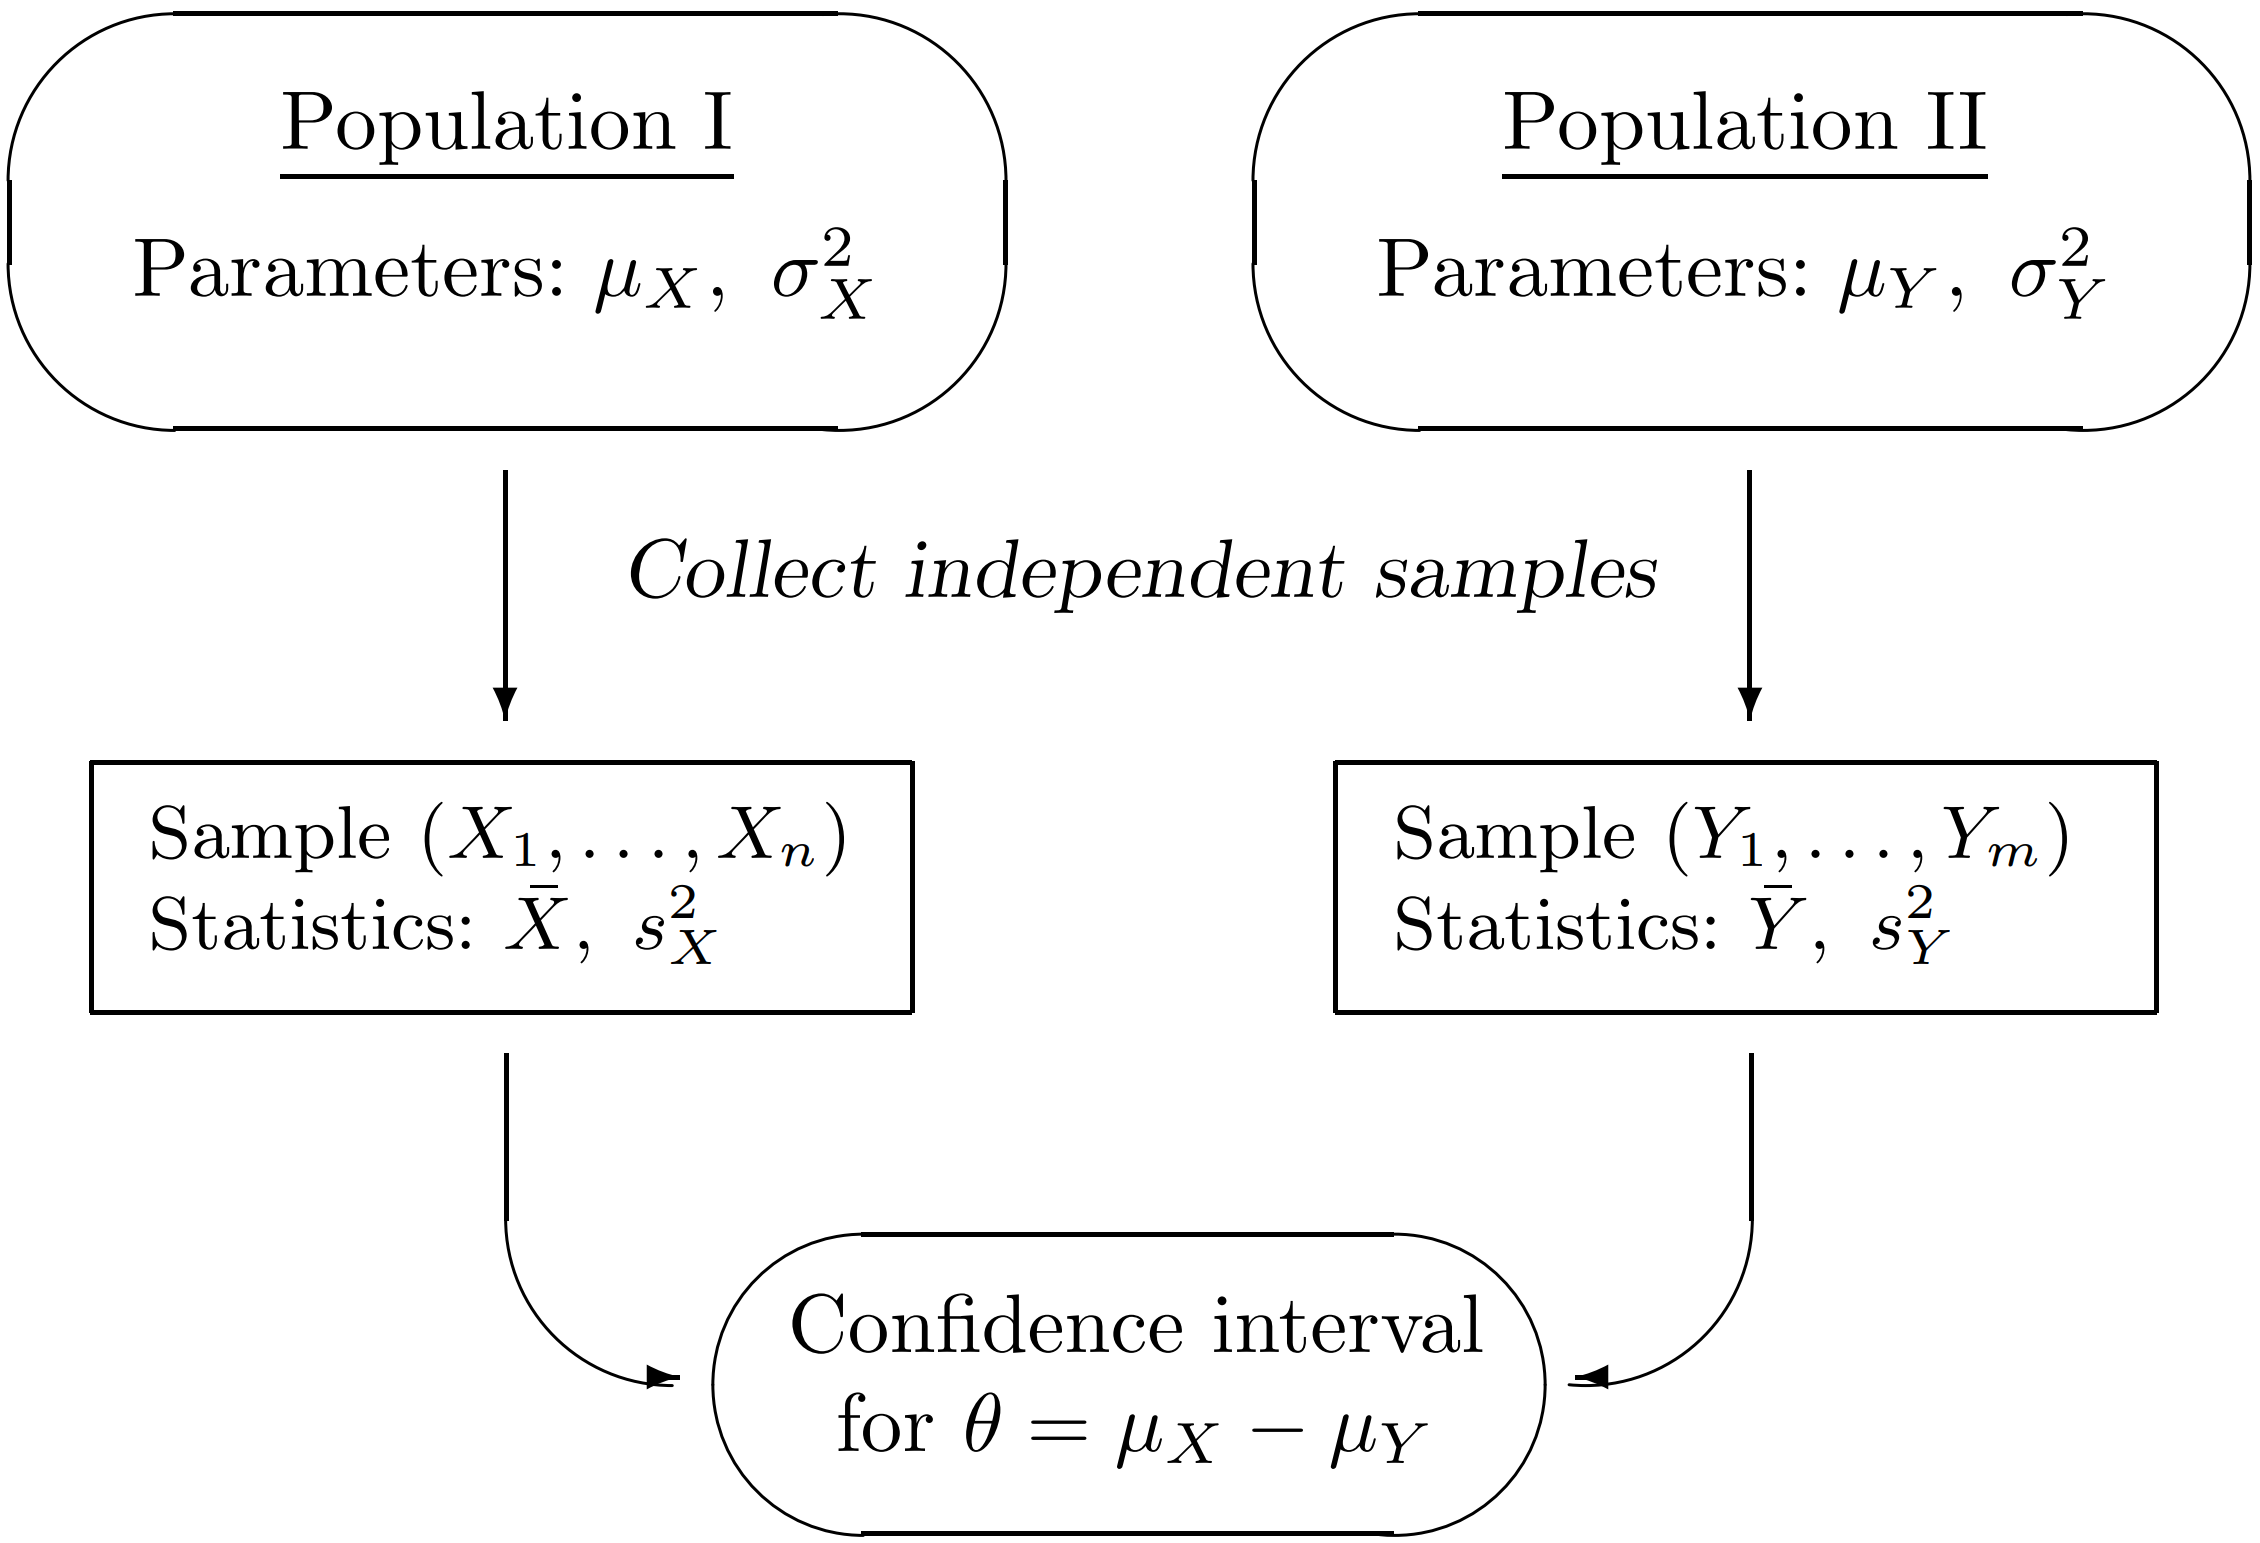
\includegraphics[width=\linewidth]{img/fig-9.4.png}
  \caption{\textit{Comparison of two populations}}
  \label{fig:9.4}
\end{figure}

Suppose that the two samples are collected \textit{independently} of each other. To construct a confidence interval for the difference between population means
\begin{equation*}
  \theta = \mu_X - \mu_Y
\end{equation*}
\noindent we complete the usual steps (a)-(e) below:
\begin{enumerate}[label=(\alph*)]
  \item Propose an estimator of $\theta$,
    \begin{equation*}
      \hat{\theta} = \bar{X} - \bar{Y}
    \end{equation*}
    It is natural to come up with this estimator because $\bar{X}$ estimates $\mu_X$ and $\bar{Y}$ estimates $\mu_Y$.
    \item Check that $\hat{\theta}$ is unbiased. Indeed,
      \begin{equation*}
        \expc{\hat{\theta}} = \expc{\bar{X} - \bar{Y}} = \expc{\bar{X}} - \expc{\bar{Y}} = \mu_X - \mu_Y = \theta
      \end{equation*}
    \item Check that $\hat{\theta}$ has a Normal or approximately Normal distribution. This is true if the observations are Normal or both sample sizes $m$ and $n$ are large.
    \item Find the standard error of $\hat{\theta}$ (using independence of $\bs{X}$ and $\bs{Y}$),
      \begin{align*}
        \sigma(\hat{\theta}) &= \sqrt{\var{\bar{X}} - \var{\bar{Y}}} = \sqrt{\var{\bar{X}} + \var{\bar{Y}}}\\
        &= \sqrt{\frac{\sigma^2_X}{n} + \frac{\sigma^2_Y}{m}}
      \end{align*}
    \item Find quantiles $\pm z_{\alpha/2}$ and compute the confidence interval according to (3). This results in the following formula.
\end{enumerate}
\begin{formula}{Confidence interval for the difference of means; known standard deviations}
  \begin{equation}
    \bar{X} - \bar{Y} \pm z_{\alpha / 2} \sqrt{\frac{\sigma^2_X}{n} + \frac{\sigma^2_Y}{m}}
  \end{equation}
\end{formula}

\begin{example}{ (Effect of an upgrade)}
  A manager evaluates effectiveness of a major hardware upgrade by running a certain process 50 times before the upgrade and 50 times after it. Based on these data, the average running time is 8.5 minutes before the upgrade, 7.2 minutes after it. Historically, the standard deviation has been 1.8 minutes, and presumably it has not changed. Construct a $90\%$ confidence interval showing how much the mean running time reduced due to the hardware upgrade.

  \textbf{Solution:}
  We have $n = m = 50$, $\sigma_X = \sigma_Y = 1.8$, $\bar{X} = 8.5$, and $\bar{Y} = 7.2$. Also, the confidence level $(1 - \alpha)$ equals 0.9, hence $\alpha / 2 = 0.05$, and $z_{\alpha/2} = 1.645$.

  The distribution of times may not be Normal; however, due to large sample sizes, the estimator 
  \begin{equation*}
    \hat{\theta} = \bar{X} - \bar{Y}
  \end{equation*}
  is approximately Normal by the Central Limit Theorem. Thus, formula (6) is applicable, and a $90\%$ confidence interval for the difference of means $(\mu_X - \mu_Y)$ is
  \begin{align*}
    8.5 - 7.2 \pm &1.645 \sqrt{(1.8)^2 \left(\frac{1}{50} + \frac{1}{50}\right)}\\
    &= 1.3 \pm 0.6 \textnormal{ or } \left[ 0.7, 1.9 \right]
  \end{align*}
  We can say that the hardware upgrade resulted in a 1.3-minute reduction of the mean running time, with a $90\%$ confidence margin of 0.6 minutes.
\end{example}

\newpage


\subsection{Selection of a Sample Size}
\label{subsec:selection-of-a-sample-size}

Formula (3) describes a confidence interval as
\begin{center}
  center $\pm$ margin
\end{center}
\noindent where
\begin{align*}
  \textnormal{center} &= \hat{\theta}\\
  \textnormal{margin} &= z_{\alpha / 2} \cdot \sigma(\hat{\theta})
\end{align*}

We can revert the problem and ask a very practical question: \textit{How large a sample should be collected to provide a certain desired precision of our estimator}?

To answer this question, we only need to solve the inequality
\begin{equation}
  \textnormal{margin} \leq \Delta
\end{equation}
in terms of $n$. Typically, parameters are estimated more accurately based on larger samples,
so that the standard error $\sigma(\hat{\theta})$ and the margin are decreasing functions of sample size $n$. Then, (7) must be satisfied for sufficiently large $n$.


\subsection{Estimating Means with a Given Precision}
\label{subsec:estimating-means-with-given-precision}

When we estimate a population mean, the margin of error is
\begin{equation*}
  \textnormal{margin} = z_{\alpha / 2} \cdot \sigma / \sqrt{n}
\end{equation*}
Solving inequality (7) for $n$ results in the following rule.
\begin{formula}{Sample size for a given precision}
  In order to attain a margin of error $\Delta$ for estimating a population mean with a confidence level $(1 - \alpha)$, a simple of size
  \begin{equation}
    n \geq \left( \frac{z_{\alpha/2} \cdot \sigma}{\Delta} \right)^2
  \end{equation}
  is required.
\end{formula}
When we compute the expression in (8), it will most likely be a fraction. Notice that we can only round it up to the nearest integer sample size. If we round it down, our margin will exceed $\Delta$.

Looking at (8), we see that a large sample will be necessary
\begin{itemize}
  \item to attain a narrow margin (small $\Delta$);
  \item to attain a high confidence level (small $\alpha$); and
  \item to control the margin under high variability of data (large $\sigma$).
\end{itemize}
In particular, we need to quadruple the sample size in order to half the margin of the interval.

\begin{example}{}
  In Example 4,  we constructed a $95\%$ confidence with the center $6.50$ and margin $1.76$ based on a sample of size $6$. Now, that was too wide, right? How large a sample do we need to estimate the population mean with a margin of at most $0.4$ units with $95\%$ confidence?

  \textbf{Solution:}
  We have $\Delta = 0.4$, $\alpha = 0.05$, and $\sigma = 2.2$ (from Example 4). By (8), we need a sample of
  \begin{equation*}
    n \geq \left( \frac{z_{0.05 / 2} \sigma}{\Delta} \right)^2 = \left( \frac{(1.960) (2.2)}{0.4} \right)^2 = 116.2
  \end{equation*}
  Keeping in mind that this is the minimum sample size that satisfies $\Delta$, and we are only allowed to round it up, we need a sample of at least 117 observations.  
\end{example}



\section{Unknown Standard Deviation}
\label{sec:unknown-standard-deviation}

A rather heavy condition was assumed when we constructed all the confidence intervals. We assumed a \textit{known standard deviation} $\sigma$ and used it in all the derived formulas.

Sometimes this assumption is perfectly valid and we may know the variance. However, generally, the population variance is \textit{unknown}. We'll then estimate it from data and see if we can still apply methods of the previous section.

Two broad situations will be considered:
\begin{itemize}
  \item large samples from any distribution,
  \item samples of any size from a Normal distribution.
\end{itemize}

\subsection{Large Samples}
\label{subsec:large-samples}

A large sample should produce a rather accurate estimator of a variance. We can then
replace the true standard error $\sigma(\hat{\theta})$ in (3) by its estimator $s(\hat{\theta})$, and obtain an approximate confidence interval
\begin{equation*}
  \hat{\theta}\ \pm\ z_{\alpha/2} \cdot s(\hat{\theta})
\end{equation*}

\begin{example}{ (Delays at nodes)}
  Internet connections are often slowed by delays at nodes. Let us determine if the delay time increases during heavy-volume times.
  
  Five hundred packets are sent through the same network between 5 pm and 6 pm (sample $\bs{X}$), and three hundred packets are sent between 10 pm and 11 pm (sample $\bs{Y}$). The early sample has a mean delay time of 0.8 sec with a standard deviation of 0.1 sec whereas the second sample has a mean delay time of 0.5 sec with a standard deviation of 0.08 sec. Construct a $99.5\%$ confidence interval for the difference between the mean delay times. \\

  \textbf{Solution:}
  We have $n = 500$, $\bar{X}$, $s_X = 0.1$; $m = 500$, $\bar{Y}$, $s_Y = 0.1$. Large sample sizes allow us to replace unknow population standard deviationsa by their estimates and use an approximately Normal distribution of sample means.

  For a confidence level of $1 - \alpha = 0.995$, we need
  \begin{equation*}
    z_{\alpha/2} = z_{0.0025} = q_{0.9975}
  \end{equation*}
  Look for the \textit{probability} 0.9975 in the body of Table A4 (from textbook) and find the corresponding value of $z$,
  \begin{equation*}
    z_{0.0025} = 2.81
  \end{equation*}
  Then, a $99.5\%$ confidence interval for the difference of mean execution times is
  \begin{align*}
    \bar{X} - \bar{Y} \ &\pm\ z_{0.0025} \sqrt{\frac{s_X^2}{n} + \frac{s_Y^2}{m}}\\
    &= (0.8 - 0.5) \ \pm\ (2.81) \sqrt{\frac{(0.1)^2}{500} + \frac{(0.08)^2}{300}}\\
    &= 0.3 \ \pm\  \textnormal{ or } \left[ 0.282,\ 0.318 \right]
  \end{align*}
\end{example}


\subsection{Confidence Intervals for Proportions}
\label{subsec:conf-inter-for-proportions}

In particular, we surely don't know the variance when we estimate a population proportion.
\begin{definition}{}
  We assume a subpopulation $A$ of items that have a certain \textit{attribute}. By the \textbf{population proportion} we mean the probability
  \begin{equation*}
    p = \prob{i \in A}
  \end{equation*}
  for a randomly selected item i to have this attribute.

  A \textbf{sample proportion}
  \begin{equation*}
    \hat{p} = \frac{\textnormal{number of sampled items from A}}{n}
  \end{equation*}
  is used to estimate $p$.
\end{definition}
\noindent Let us use the \textit{indicator} variables
\begin{equation*}
  X_i = \begin{cases}
    1 &\textnormal{if } i \in A\\
    0 &\textnormal{if } i \notin A\\
  \end{cases}
\end{equation*}
Each $X_i$ has Bernoulli distribution with parameter $p$. In particular
\begin{align*}
  \expc{X_i} = p &&\textnormal{and}& &\var{X_i} = p (1 - p)
\end{align*}
Also,
\begin{equation*}
  \hat{p} = \frac{1}{n} \sum_{i=1}^{n} X_i
\end{equation*}
is nothing but a sample of $X_i$.

\noindent Therefore,
\begin{align*}
  \expc{\hat{p}} = p &&\textnormal{and}& &\var{\hat{p}} = \frac{p (1 - p)}{n}
\end{align*}

\vspace*{\fill}
\columnbreak

\noindent We conclude that
\begin{enumerate}
  \item a sample proportion $\hat{p}$ is unbiased for the population proportion $p$;
  \item it has approximately Normal distribution for large samples, because it has a form of
  a sample mean;
  \item when we construct a confidence interval for $p$, we do not know the standard deviation
  Std($\hat{p}$).
\end{enumerate}

Indeed, knowing the standard deviation is equivalent to knowing p, and if we know p, why
would we need a confidence interval for it?

Thus, we estimate the unknown standard error
\begin{equation*}
  \sigma(\hat{p}) = \sqrt{\frac{p (1-p)}{n}}
\end{equation*}
by
\begin{equation*}
  s(\hat{p}) = \sqrt{\frac{\hat{p} (1 - \hat{p})}{n}}
\end{equation*}
and use it in the general formula
\begin{equation*}
  \hat{p}\ \pm\ z_{\alpha/2} \cdot s(\hat{p})
\end{equation*}
to construct an approximate $(1 - \alpha)100\%$ confidence interval.
\begin{formula}{Confidence interval for a population proportion}
  \begin{equation*}
    \hat{p} \ \pm\ z_{\alpha/2} \sqrt{\frac{\hat{p} (1 - \hat{p})}{n}}
  \end{equation*}
\end{formula}

Similarly, we can construct a confidence interval for the difference between two proportions. In two populations, we have proportions $p_1$ and $p_2$ of items with an attribute. Independent samples of size $n_1$ and $n_2$ are collected, and both parameters are estimated by sample proportions $\hat{p_1}$ and $\hat{p_2}$.

Summarizing, we have
\begin{align*}
  \textnormal{Parameter of interest:} &\theta = p_1 - p_2 \\
  \textnormal{Estimated by:}          &\hat{\theta} = \hat{p_1} - \hat{p_2} \\
  \textnormal{Its standard error:}    &\sigma(\hat{\theta}) = \sqrt{\frac{p_1 (1 - p_1)}{n_1} + \frac{p_2 (1- p_2)}{n_2}} \\
  \textnormal{Estimated by:}          &s(\hat{\theta}) = \sqrt{\frac{\hat{p_1} (1 - \hat{p_1})}{n_1} + \frac{\hat{p_2} (1- \hat{p_2})}{n_2}}
\end{align*}

\begin{formula}{Confidence interval for the difference of proportions}
  \begin{equation*}
    \hat{p_1} - \hat{p_2} \ \pm \ z_{\alpha/2} \sqrt{\frac{\hat{p_1} (1 - \hat{p_1})}{n_1} + \frac{\hat{p_2} (1 - \hat{p_2})}{n_2}}
  \end{equation*}
\end{formula}

\begin{example}{ (Pre-election poll)}
  A candidate prepares for the local elections. During his campaign, 42 out of 70 randomly selected people in town A and 59 out of 100 randomly selected people in town B showed they would vote for this candidate. Estimate the difference in support that this candidate is getting in towns A and B with $95\%$ confidence. Can we state affirmatively that the candidate gets a stronger support in town A? \\

  \textbf{Solution:}
  We have $n_1 = 70$, $n_2 = 100$, $\hat{p_1} = 42/70 = 0.6$, and $\hat{p_2} = 59/100 = 0.59$. For the confidence interval, we have
  \begin{equation*}
    \textnormal{center} = \hat{p_1} - \hat{p_2} = 0.01
  \end{equation*}
  and
  \begin{align*}
    \textnormal{margin} &= z_{0.05/2} \sqrt{\frac{\hat{p_1} (1 - \hat{p_1})}{n_1} + \frac{\hat{p_2} (1 - \hat{p_2})}{n_2}}\\
    &= (1.960) \sqrt{\frac{(0.6) (0.4)}{70} + \frac{(0.59) (0.41)}{100}} = 0.15
  \end{align*}
  Then
  \begin{equation*}
    0.01 \ \pm \ 0.15 = \left[ -0.14,\ 0.16 \right]
  \end{equation*}
  is a $95\%$ confidence interval for the difference in support ($p_1 - p_2$) in the two towns.\\

  So, is the support stronger in town A? On one hand, the estimator $\hat{p_1} - \hat{p_2} = 0.01$ suggests that the support is $1\%$ higher in town A than in town B. On the other hand, the difference could appear positive just because of a sampling error. As we see, the $95\%$ confidence interval includes a large range of negative values too. Therefore, the obtained data \textit{does not} indicate affirmatively that the support in town A is stronger.
\end{example}


\subsection{Estimating Proportions with a Given Precision}
\label{subsec:est-propor-given-precision}

Our confidence interval for a population proportion has a margin
\begin{equation*}
  \textnormal{margin} = z_{\alpha/2} \sqrt{\frac{\hat{p} (1 - \hat{p})}{n}}
\end{equation*}
A standard way of finding the sample size that provides the desired margin $\Delta$ is to solve the inequality
\begin{align*}
  \textnormal{margin} \leq \Delta &&\textnormal{or}&& n \geq \hat{p} (1 - \hat{p}) \left( \frac{z_{\alpha/2}}{\Delta} \right)^2
\end{align*}
However, this inequality includes $\hat{p}$. To know $\hat{p}$, we first need to collect a sample, but to know the sample size, we first need to know $\hat{p}$!

Since $\hat{p} (1 - \hat{p})$ does not exceed 0.25, we can replace this unknown by 0.25 and find a sample size $n$, perhaps larger than we actually need, that will ensure that we estimate $\hat{p}$ with a margin not exceeding $\Delta$. That is, choose a sample size
\begin{equation*}
  n \geq 0.25 \left( \frac{z_{\alpha / 2}}{\Delta} \right)^2
\end{equation*}

\begin{example}{}
  A sample of size
  \begin{equation*}
    n \geq 0.25 \left( \frac{1.960}{0.1} \right)^2 = 96.04
  \end{equation*}
  that is, at least 97 observations always guarantees that a populaiton proportion is estimated with an error of at most 0.1 with a $95\%$ confidence.
\end{example}


\subsection{Small Samples: Student's \textit{t} distribution}
\label{subsec:small-samples}

Having a small sample, we can no longer pretend that a sample standard deviation $s$ is an accurate estimator of the population standard deviation $\sigma$. Then, how should we adjust the confidence interval when we replace $\sigma$ by $s$, or more generally, when we replace the standard error $\sigma(\hat{\theta})$ by its estimator $s(\hat{\theta})$?

A famous solution was proposed by \textit{William Gosset} (1876–1937), he derived the \textbf{T-distribution}.

He replaced the true but unknown standard error of $\hat{\theta}$ by its estimator $s(\hat{\theta})$ and concluded that the \textbf{T-ratio}
\begin{equation*}
  t = \frac{\hat{\theta} - \theta}{s(\hat{\theta})}
\end{equation*}
the \textit{ratio} of two random variables, no longer has a Normal distribution!

For the problem of estimating the mean based on $n$ Normal observations $X_1,\ \ldots,\ X_n$, this was \textbf{T-distribution} with $(n - 1)$ \textit{degrees of freedom}. Table A5 (from textbook) gives critical values $t_{\alpha}$ of the T-distribution that we'll use for confidence intervals.

So, using \textit{T-distribution} instead of Standard Normal and estimated standard error instead of the unknown true one, we obtain the confidence interval for the population mean.

\begin{formula}{Confidence interval for the mean $\sigma$ is unknown}
  \begin{equation}
    \bar{X} \ \pm\ t_{\alpha/2} \frac{s}{\sqrt{n}}
  \end{equation}
  where $t_{\alpha/2}$ is a critical value from T-distribution with $n - 1$ degrees of freedom.
\end{formula}

The density of \textit{Student's T-distribution} is a bell-shaped symmetric curve that can be easily confused with Normal. Comparing with the Normal density, \textit{its peak is lower and its tails are thicker}. Therefore, a larger number $t_{\alpha}$ is generally needed to cut area $\alpha$ from the right tail. That is
\begin{equation*}
  t_{\alpha} > z_{\alpha}
\end{equation*}
for small $\alpha$. As a consequence, the confidence interval (9) is wider than the interval (5) for the case of known $\sigma$. This wider margin is the price paid for not knowing the standard deviation $\sigma$. When we lack a certain piece of information, we cannot get a more accurate estimator.

\vspace*{\fill}
\columnbreak

However, we see in Table A5 that
\begin{equation*}
  t_{\alpha} \ra z_{\alpha}
\end{equation*}
as the number of degrees of freedom $\nu$ tends to infinity. Indeed, having a large sample (hence, large $\nu = n - 1$), we can count on a very accurate estimator of $\sigma$, and thus, the confidence interval is almost as narrow as if we knew $\sigma$ in this case.

\textbf{Degrees of freedom $\nu$} is the parameter of T-distribution controlling the shape of the T-density curve. Its meaning is the dimension of a vector used to estimate the variance. Here we estimate $\sigma^2$ by a sample variance
\begin{equation*}
  s^2 = \frac{1}{n - 1} \sum_{i=1}^{n} (X_i - \bar{X})^2
\end{equation*}
and thus, we use a vector
\begin{equation*}
  \bs{X'} = (X_1 - \bar{X},\ \ldots,\ X_n - \bar{X})
\end{equation*}
The initial vector $\bs{X} = (X_1,\ \ldots,\ X_n)$ has dimension $n$; therefore, it has $n$ degrees of freedom. However, when the sample mean $\bar{X}$ is subtracted from each observation, there appears a linear relation among the elements,
\begin{equation*}
  \sum_{i=1}^{n} (X_i - \bar{X}) = 0
\end{equation*}
We lose 1 degree of freedom due to this constraint; the vector $\bs{X'}$ belongs to an $(n - 1)$.

In many similar problems, degrees of freedom can be computed as
\begin{table}[H]
  \centering
  \begin{tabular}{p{2cm} c p{2cm} c p{2cm} r}
    number of degrees of freedom & $=$ & sample size & $-$ & number of estimated location parameters & (10) \\
  \end{tabular}
\end{table}


\subsection{Comparison of Two Populations with Unknown Variances}
\label{subsec:comp-two-pop-unknown-var}
\setcounter{equation}{10}

We now construct a confidence interval for the difference of two means $\mu_X - \mu_Y$, comparing the population of $X$'s with the population of $Y$'s.

Again, independent random samples are collected,
\begin{align*}
  \bs{X} = (X_1,\ \ldots,\ X_n) &&\textnormal{and}&& \bs{Y} = (Y_1,\ \ldots,\ Y_m)
\end{align*}
one from each population, as in Figure 4. This time, however, population variances $\sigma^2_X$ and $\sigma^2_Y$ are unknown to us, and we use their estimates.

Two important cases need to be considered here. In one case, there exists an exact and simple solution based on T-distribution. The other case suddenly appears to be a famous Behrens-Fisher problem, where no exact solution exists, and only approximations are available.

\vspace*{\fill}
\columnbreak

\subsubsection{Case 1. Equal Variances}

Suppose there are reasons to assume that the two populations have equal variances,
\begin{equation*}
  \sigma^2_X = \sigma^2_Y = \sigma^2
\end{equation*}
For example, two sets of data are collected with the same measurement device, thus, measurements have different means but the same precision. In this case, there is only one variance $\sigma^2$ to estimate instead of two. We should use both samples $\bs{X}$ and $\bs{Y}$ to estimate their common variance. This estimator of $\sigma^2$ is called a \textbf{pooled sample variance}, and it is computed as
\begin{align}
  s_p^2 &= \frac{\dsum_{i=1}^{n} (X_i - \bar{X})^2 + \dsum_{i=1}^{n} (Y_i - \bar{Y})^2}{n + m - 2} \nonumber \\
  &= \frac{(n-1) s_X^2 + (n-1) s_Y^2}{n + m - 2}
\end{align}
Substituting this variance estimator in (6) for $\sigma^2_X$ and $\sigma^2_Y$, we get the following confidence interval.
\begin{formula}{Confidence interval for the difference of means; equal, unknown standard deviations}
  \begin{equation*}
    \bar{X} - \bar{Y} \ \pm\ t_{\alpha/2} s_p \sqrt{\frac{1}{n} + \frac{1}{m}}
  \end{equation*}
  where $s_p$ is the pooled standard deviation, a root of the pooled variance in (11) and $t_{\alpha/2}$ is a critical value from T-distribution with $(n + m - 2)$ degrees of freedom.
\end{formula}

\subsubsection{Case 2. Unequal Variances}

The most difficult case is when both variances are unknown and unequal. Confidence estimation of $\mu_X - \mu_Y$ in this case is known as the \textit{Behrens-Fisher} problem. Certainly, we can replace unknown variances $\sigma^2_X$, $\sigma^2_Y$ by their estimates $s^2_X$, $s^2_Y$ and form a T-ratio
\begin{equation*}
  t = \frac{(\bar{X} - \bar{Y}) - (\mu_X - \mu_Y)}{\sqrt{\dfrac{s_X^2}{n} + \dfrac{s_Y^2}{m}}}
\end{equation*}
However, it won't have a T-distribution.

An approximate solution was proposed in the 1940s by Franklin E. Satterthwaite. Satterthwaite used the method of moments to estimate degrees of freedom $\nu$ of a T-distribution that is ``closest'' to this T-ratio. This number depends on unknown variances. Estimating them by sample variances, he obtained the formula that is now known as \textit{Satterthwaite approximation}
\begin{equation}
  \nu = \dfrac{\left( \dfrac{s_X^2}{n} + \dfrac{s_Y^2}{m} \right)^2}{\dfrac{s_X^4}{n^2(n-1)} + \dfrac{s_Y^4}{m^2(m-1)}}
\end{equation}
This number of degrees of freedom often appears non-integer. There are T-distributions with non-integer $\nu$. To use Table A5, just take the closest $\nu$ that is given in that table.

\vspace*{\fill}
\columnbreak

Formula (12) is widely used for t-intervals and t-tests.
\begin{formula}{Confidence interval for the difference of means; unequal, unknown standard deviation}
  \begin{equation*}
    \bar{X} - \bar{Y} \ \pm \ t_{\alpha/2} \sqrt{\frac{s_X^2}{n} + \frac{s_Y^2}{m}}
  \end{equation*}
  where $t_{\alpha/2}$ is a critical value from T-distribution with $\nu$ degrees of freedom given by formula (12).
\end{formula}

\textbf{\textit{Check the examples of 9.3.4 from book.}}



\section{Hypothesis Testing}
\label{sec:hypothesis-testing}

\subsection{Hypothesis and Alternative}
\label{subsec:hypothesis-alternative}

To begin, we need to state exactly what we are testing. These are hypothesis and alternative.

\begin{formula}{NOTATION}
  \begin{center}
    $\begin{aligned}
      &H_0 = \textnormal{hypothesis (the null hypothesis)}\\
      &H_A = \textnormal{alternative (the alternative hypothesis)}
    \end{aligned}$
  \end{center}
\end{formula}

$H_0$ and $H_A$ are simply two mutually exclusive statements. Each test results either in acceptance of $H_0$ or its rejection in favor of $H_A$.
\begin{definition}{}
  Alternative of the type $H_A$: $\mu \neq \mu_0$ covering regions on both sides of the hypothesis ($H_0$: $\mu = \mu_0$) is a \textbf{two-sided alternative}.\\
  Alternative $H_A$: $\mu < \mu_0$ covering the region to the left of $H_0$ is \textbf{one-sided, left-tail.}\\
  Alternative $H_A$: $\mu > \mu_0$ covering the region to the right of $H_0$ is \textbf{one-sided, right-tail.}
\end{definition}

\textbf{\textit{\underline{Check the examples 9.22, 9.23, 9.24.}}}


\subsection{Type I and Type II errors: Level of Significance}
\label{subsec:type-1-2-errors}

When testing hypotheses, we realize that all we see is a random sample. Therefore, with all the best statistics skills, our decision to accept or to reject $H_0$ may still be wrong
\begin{table}[H]
  \centering
  \renewcommand{\arraystretch}{2}
  \begin{tabular}{|c|c|c|} 
  \cline{2-3}
  \multicolumn{1}{c|}{} & \multicolumn{2}{c|}{\textbf{Result of the test}}  \\ 
  \cline{2-3}
  \multicolumn{1}{c|}{} & Reject $H_0$  & Accept $H_0$               \\ 
  \hline
  $H_0$ is true          & Type I error & correct                   \\ 
  \hline
  $H_0$ is false         & correct      & Type II error             \\
  \hline
  \end{tabular}
\end{table}
\begin{definition}{}
  A \textbf{type I error} occurs when we reject the true null hypothesis.\\

  A \textbf{type II error} occurs when we accept the false null hypothesis.
\end{definition}

A type I error is often considered \textit{more dangerous and undesired} than a type II error. For this reason,  we shall design tests that bound the probability of type I error by a preassigned small number $\alpha$. Under this condition, we may want to minimize the probability of type II error.

\begin{definition}{}
  Probability of a type I error is the \textbf{significance level} of a test,
  \begin{equation*}
    \alpha = \prob{\textnormal{reject } H_0\ |\ H_0 \textnormal{ is true}}
  \end{equation*}
  Probability of rejecting a false hypothesis is the \textbf{power of the test},
  \begin{equation*}
    p(\theta) = \prob{\textnormal{reject } H_0\ |\ H_A \textnormal{ is true}}
  \end{equation*}
  It is usually a function of the parameter $\theta$ because the alternative hypothesis includes a set of parameter values. Also, the power is the probability to avoid a Type II error.
\end{definition}


\subsection{Level \texorpdfstring{$\alpha$}{alpha} Tests: General Approach}
\label{subsec:level-alpha-tests}

A standard algorithm for a level $\alpha$ test of a hypothesis $H_0$ against an alternative $H_A$ consists of 3 steps.

\subsubsection*{Step 1. Test Statistic}

Testing hypothesis is based on a \textbf{test statistic} $T$ , a quantity computed from the data that has some known, tabulated distribution $F_0$ if the hypothesis $H_0$ is true.

\subsubsection*{Step 2. Acceptance Region and Rejection Region}

Next, we consider the \textbf{null distribution} $F_0$. This is the distribution of test statistic $T$ when the hypothesis $H_0$ is true. If it has a density $f_0$, then the whole area under the density curve is 1, and we can always find a portion of it whose area is $\alpha$, as shown in Figure 5. It is called \textbf{rejection region} ($\mathcal{R}$).

The remaining part, the complement of the rejection region, is called \textbf{acceptance region} ($\mathcal{A = \overline{R}}$). By the complement rule, its area is ($1 - \alpha$).

\subsubsection*{Step 3. Result and Its Interpretation}

Accept the hypothesis $H_0$ if the test statistic $T$ belongs to the acceptance region. Reject $H_0$ in favor of the alternative $H_A$ if $T$ belongs to the rejection region.

\begin{figure}[H]
  \centering
  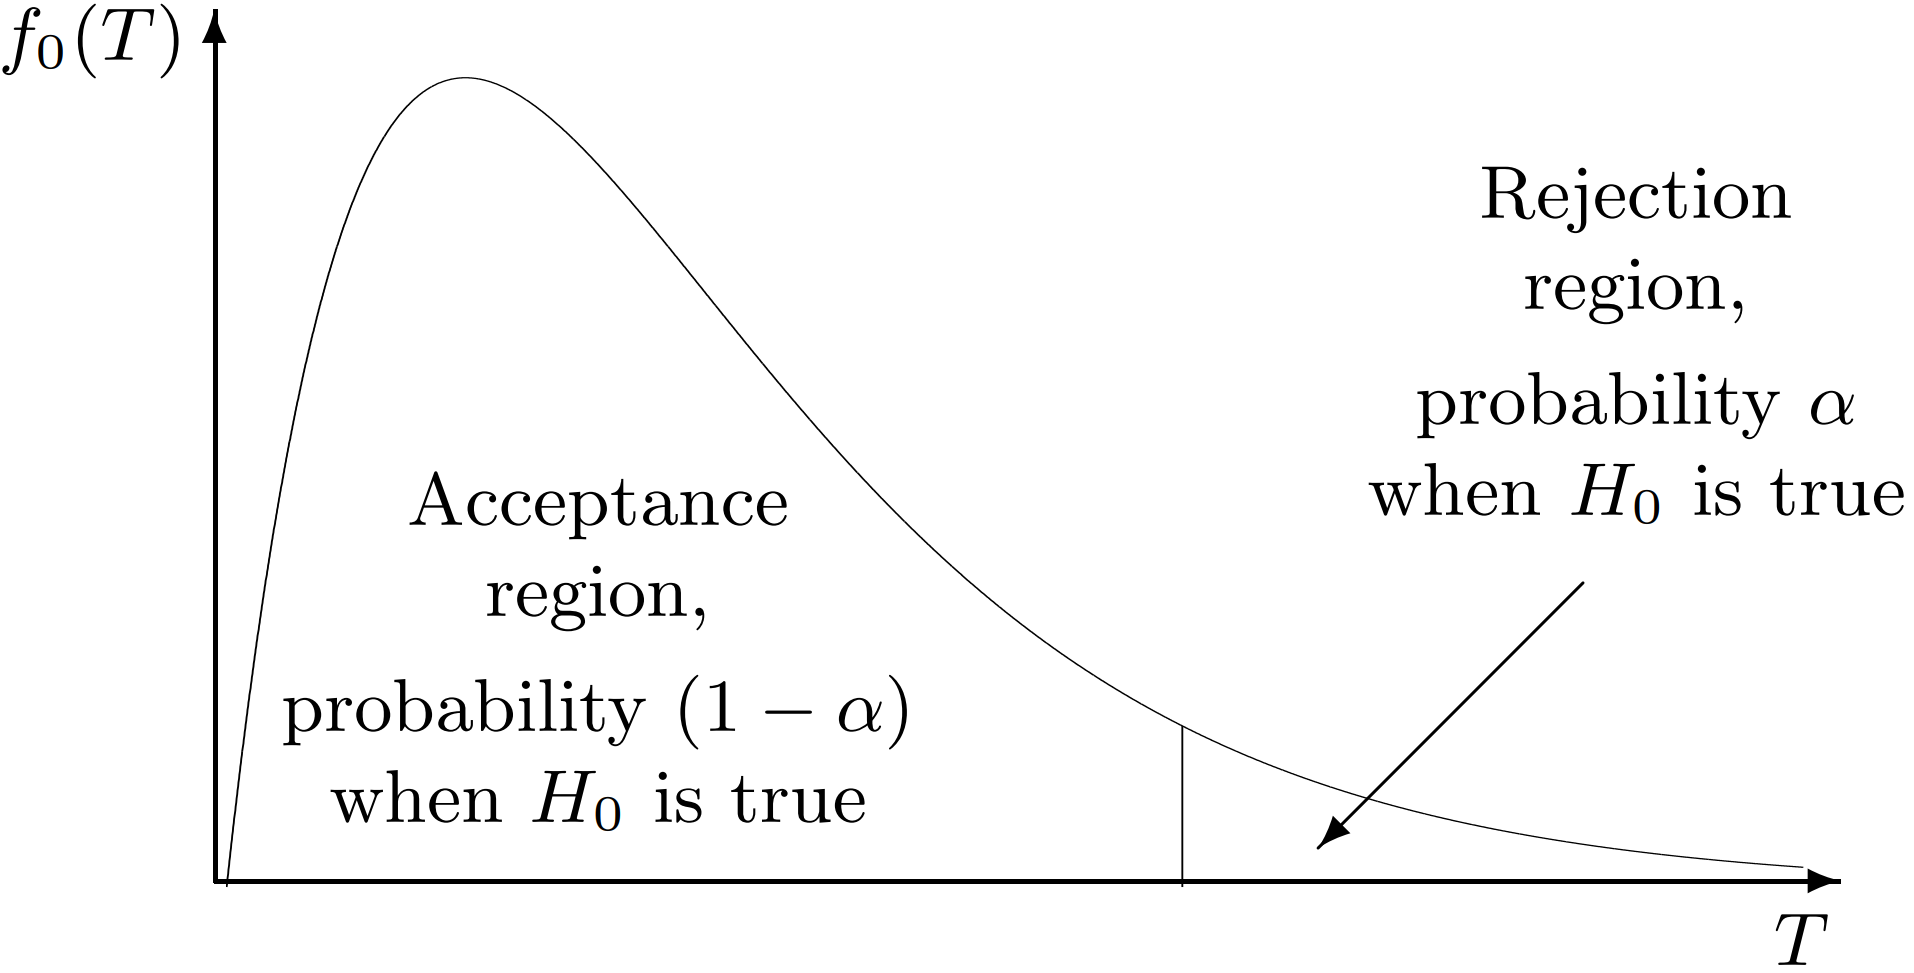
\includegraphics[width=\linewidth]{img/fig-9.6.png}
  \caption{}
  \label{fig:9.6}
\end{figure}


\subsection{Rejection Regions and Power}
\label{subsec:rejection-region-and-power}

\begin{figure}[H]
  \centering
  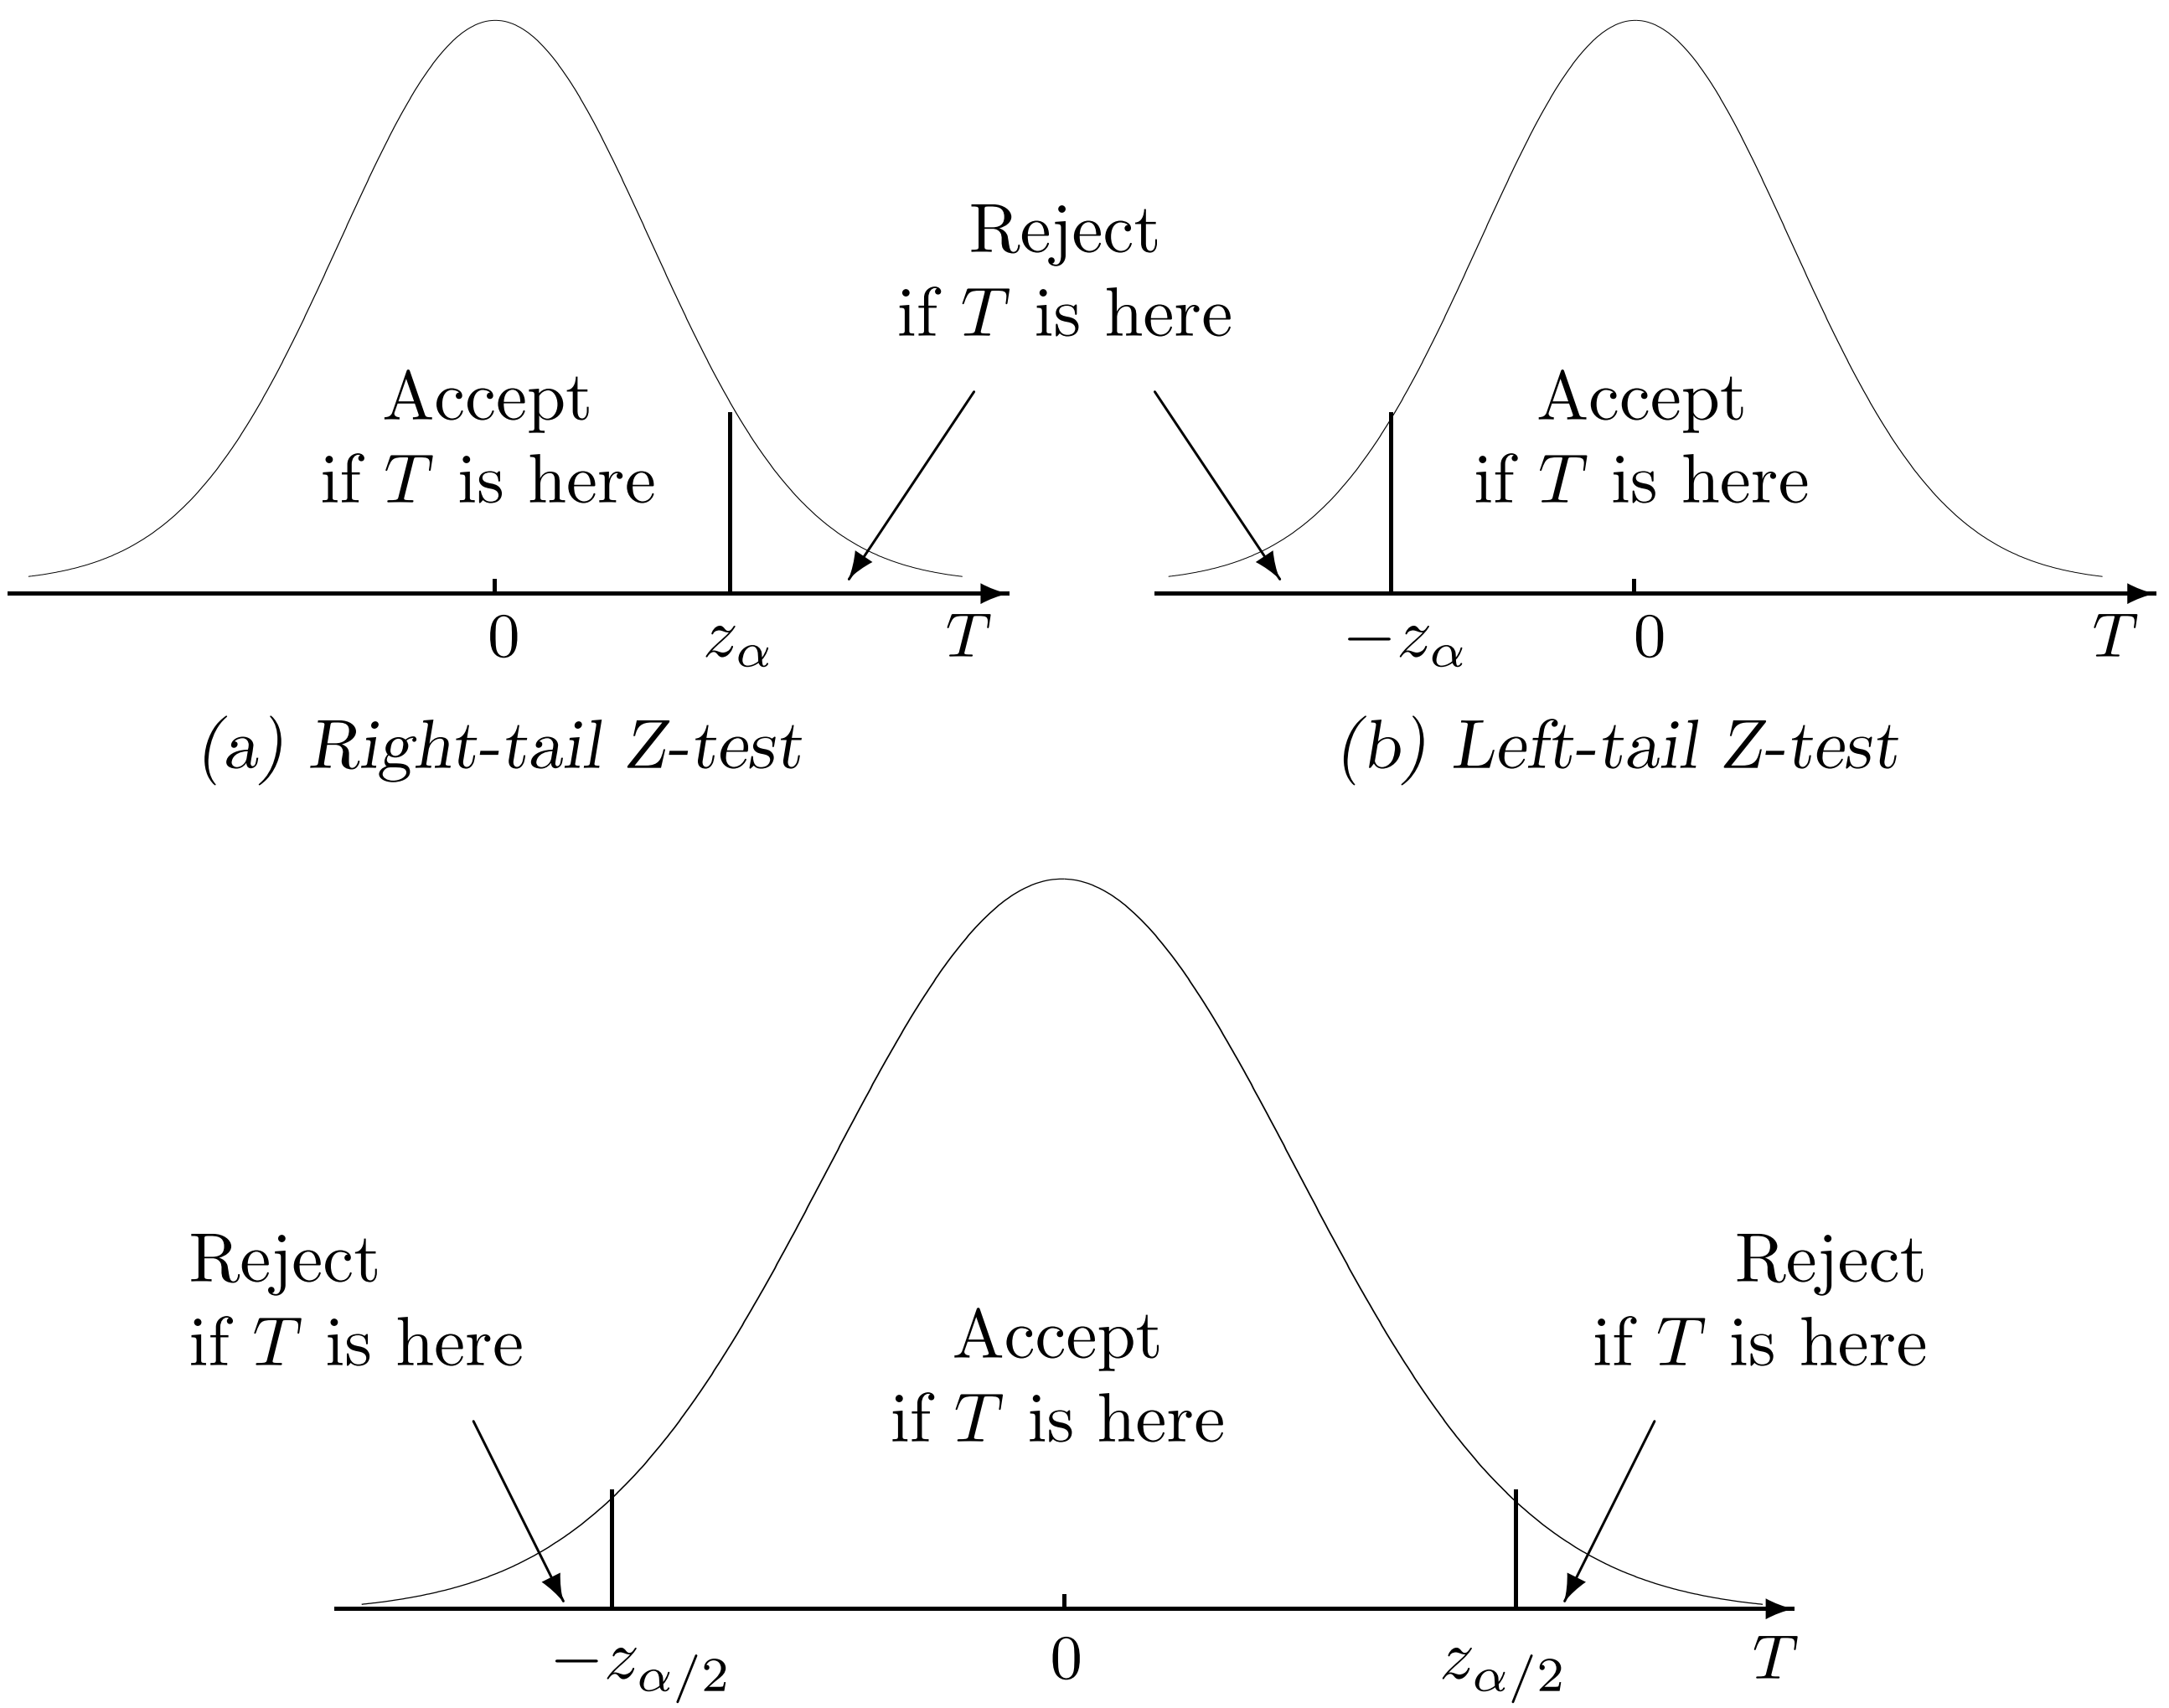
\includegraphics[width=\linewidth]{img/fig-9.7.png}
  \caption{\textit{Acceptance and rejection regions for a $Z$-test with (a) a one-sided right-tail alternative; (b) a one-sided left-tail alternative; (c) a two-sided alternative.}}
  \label{fig:9.7}
\end{figure}

\begin{itemize}[leftmargin=.6cm]
  \item For a \textbf{right-tail alternative}, the rejection region $\mathcal{R}$ should consist of large values of $T$ . Choose $\mathcal{R}$ on the right, $\mathcal{A}$ on the left (Figure 6a).
  \item For a \textbf{left-tail alternative}, the rejection region $\mathcal{R}$ should consist of small values of $T$ . Choose $\mathcal{R}$ on the left, $\mathcal{A}$ on the right (Figure 6b).
  \item For a \textbf{two-sided alternative}, the rejection region $\mathcal{R}$ should consist of very small and very large values of $T$ . Let $\mathcal{R}$ consist of two extreme regions, while $\mathcal{A}$ covers the middle (Figure 6c).
\end{itemize}


\subsection{\textit{Z}-Test: Standard Normal Null Distribution}
\label{subsec:z-test}
\setcounter{equation}{13}

An important case, in terms of a large number of applications, is when the null distribution of the test statistic is \textit{Standard Normal}.

The test in this case is called a \textbf{Z-test}, and the test statistic is usually denoted by $Z$.

\begin{enumerate}[label=(\alph*)]
  \item A level $\alpha$ test with a \textbf{right-tail alternative} should
    \begin{equation}
      \begin{cases}
        \textnormal{reject } H_0 &\textnormal{if } Z \geq z_{\alpha}\\
        \textnormal{accepts } H_0 &\textnormal{if } Z < z_{\alpha}\\
      \end{cases}
    \end{equation}
    The rejection region in this case consists of large values of $Z$ only,
    \begin{align*}
      \mathcal{R} = \left[ z_{\alpha},\ +\infty \right), & &\mathcal{A} = \left( -\infty,\ z_{\alpha} \right)
    \end{align*}
    Under the null hypothesis, $Z$ belongs to $\mathcal{A}$ and we reject the null hypothesis with probability
    \begin{equation*}
      \prob{T \geq z_{\alpha}\ |\ H_0} = 1 - \Phi(z_{\alpha}) = \alpha
    \end{equation*}
    making the probability of false rejection (type I error) equal $\alpha$.

    For example, we use this acceptance region to test the population mean,
    \begin{align*}
      H_0\ :\ \mu = \mu_0 &&\textnormal{vs}&& H_A\ :\ \mu > \mu_0
    \end{align*}
  
  \item With a \textbf{left-tail alternative} should
    \begin{equation}
      \begin{cases}
        \textnormal{reject } H_0 &\textnormal{if } Z \leq -z_{\alpha}\\
        \textnormal{accepts } H_0 &\textnormal{if } Z > -z_{\alpha}\\
      \end{cases}
    \end{equation}
    The rejection region consists of smal values of $Z$ only,
    \begin{align*}
      \mathcal{R} = \left( -\infty,\ -z_{\alpha} \right], & &\mathcal{A} = \left( -z_{\alpha},\ +\infty \right)
    \end{align*}
    Similarly, $\prob{Z \in \mathcal{R}} = \alpha$ under $H_0$; thus, the probability of type I error equals $\alpha$. For example, this is how we should test
    \begin{align*}
      H_0\ :\ \mu = \mu_0 &&\textnormal{vs}&& H_A\ :\ \mu < \mu_0
    \end{align*}

  \item With a \textbf{two-sided alternative}, we
    \begin{equation}
      \begin{cases}
        \textnormal{reject } H_0 &\textnormal{if } |Z| \geq z_{\alpha/2}\\
        \textnormal{accepts } H_0 &\textnormal{if } |Z| < z_{\alpha/2}\\
      \end{cases}
    \end{equation}
    The rejection region consists of very small and very large values of $Z$,
    \begin{align*}
      \mathcal{R} = \left( -\infty,\ z_{\alpha} \right] \cup \left[ z_{\alpha/2},\ +\infty \right), & &\mathcal{A} = \left( -z_{\alpha/2},\ z_{\alpha/2} \right)
    \end{align*}
    Again, the probability of type I error equals $\alpha$. For example, we use this test for
    \begin{align*}
      H_0\ :\ \mu = \mu_0 &&\textnormal{vs}&& H_A\ :\ \mu \neq \mu_0
    \end{align*}
\end{enumerate}

This is easy to remember:
\begin{itemize}
  \item for a two-sided test, divide $\alpha$ by two and use $z_{\alpha/2}$;
  \item for a one-sided test, use $z_{\alpha}$ keeping in mind that the rejection region consists of just one piece.
\end{itemize}

Now consider testing a hypothesis about a population parameter $\theta$. Suppose that its estimator $\hat{\theta}$ has Normal distribution, at least approximately, and we know $\expc{\hat{\theta}}$ and $\var(\hat{\theta})$ if the hypothesis is true.

Then the test statistic
\begin{equation}
  Z = \frac{\hat{\theta} - \expc{\hat{\theta}}}{\sqrt{\var{\hat{\theta}}}}
\end{equation}
has Standard Normal distribution, and we can use (14), (15), and (16) to construct acceptance and rejection regions for a level $\alpha$ test. We call $Z$ a \textbf{Z-statistic}.


\subsection{\textit{Z}-Test for Means and Proportions}
\label{subsec:z-test-for-means-proportions}

As we already know,
\begin{itemize}
  \item sample means have Normal distribution when the distribution of data is Normal;
  \item sample means have approximately Normal distribution when they are computed from large samples (the distribution of data can be arbitrary);
  \item sample proportions have approximately Normal distribution when they are computed from large samples;
  \item this extends to differences between means and between proportions
\end{itemize}

For all these cases, we can use a Z-statistic (17) and rejection regions (14)-(16) to design powerful level $\alpha$ tests.

Z-tests are summarized in Table 1.

\end{multicols}

\begin{figure}[H]
  \centering
  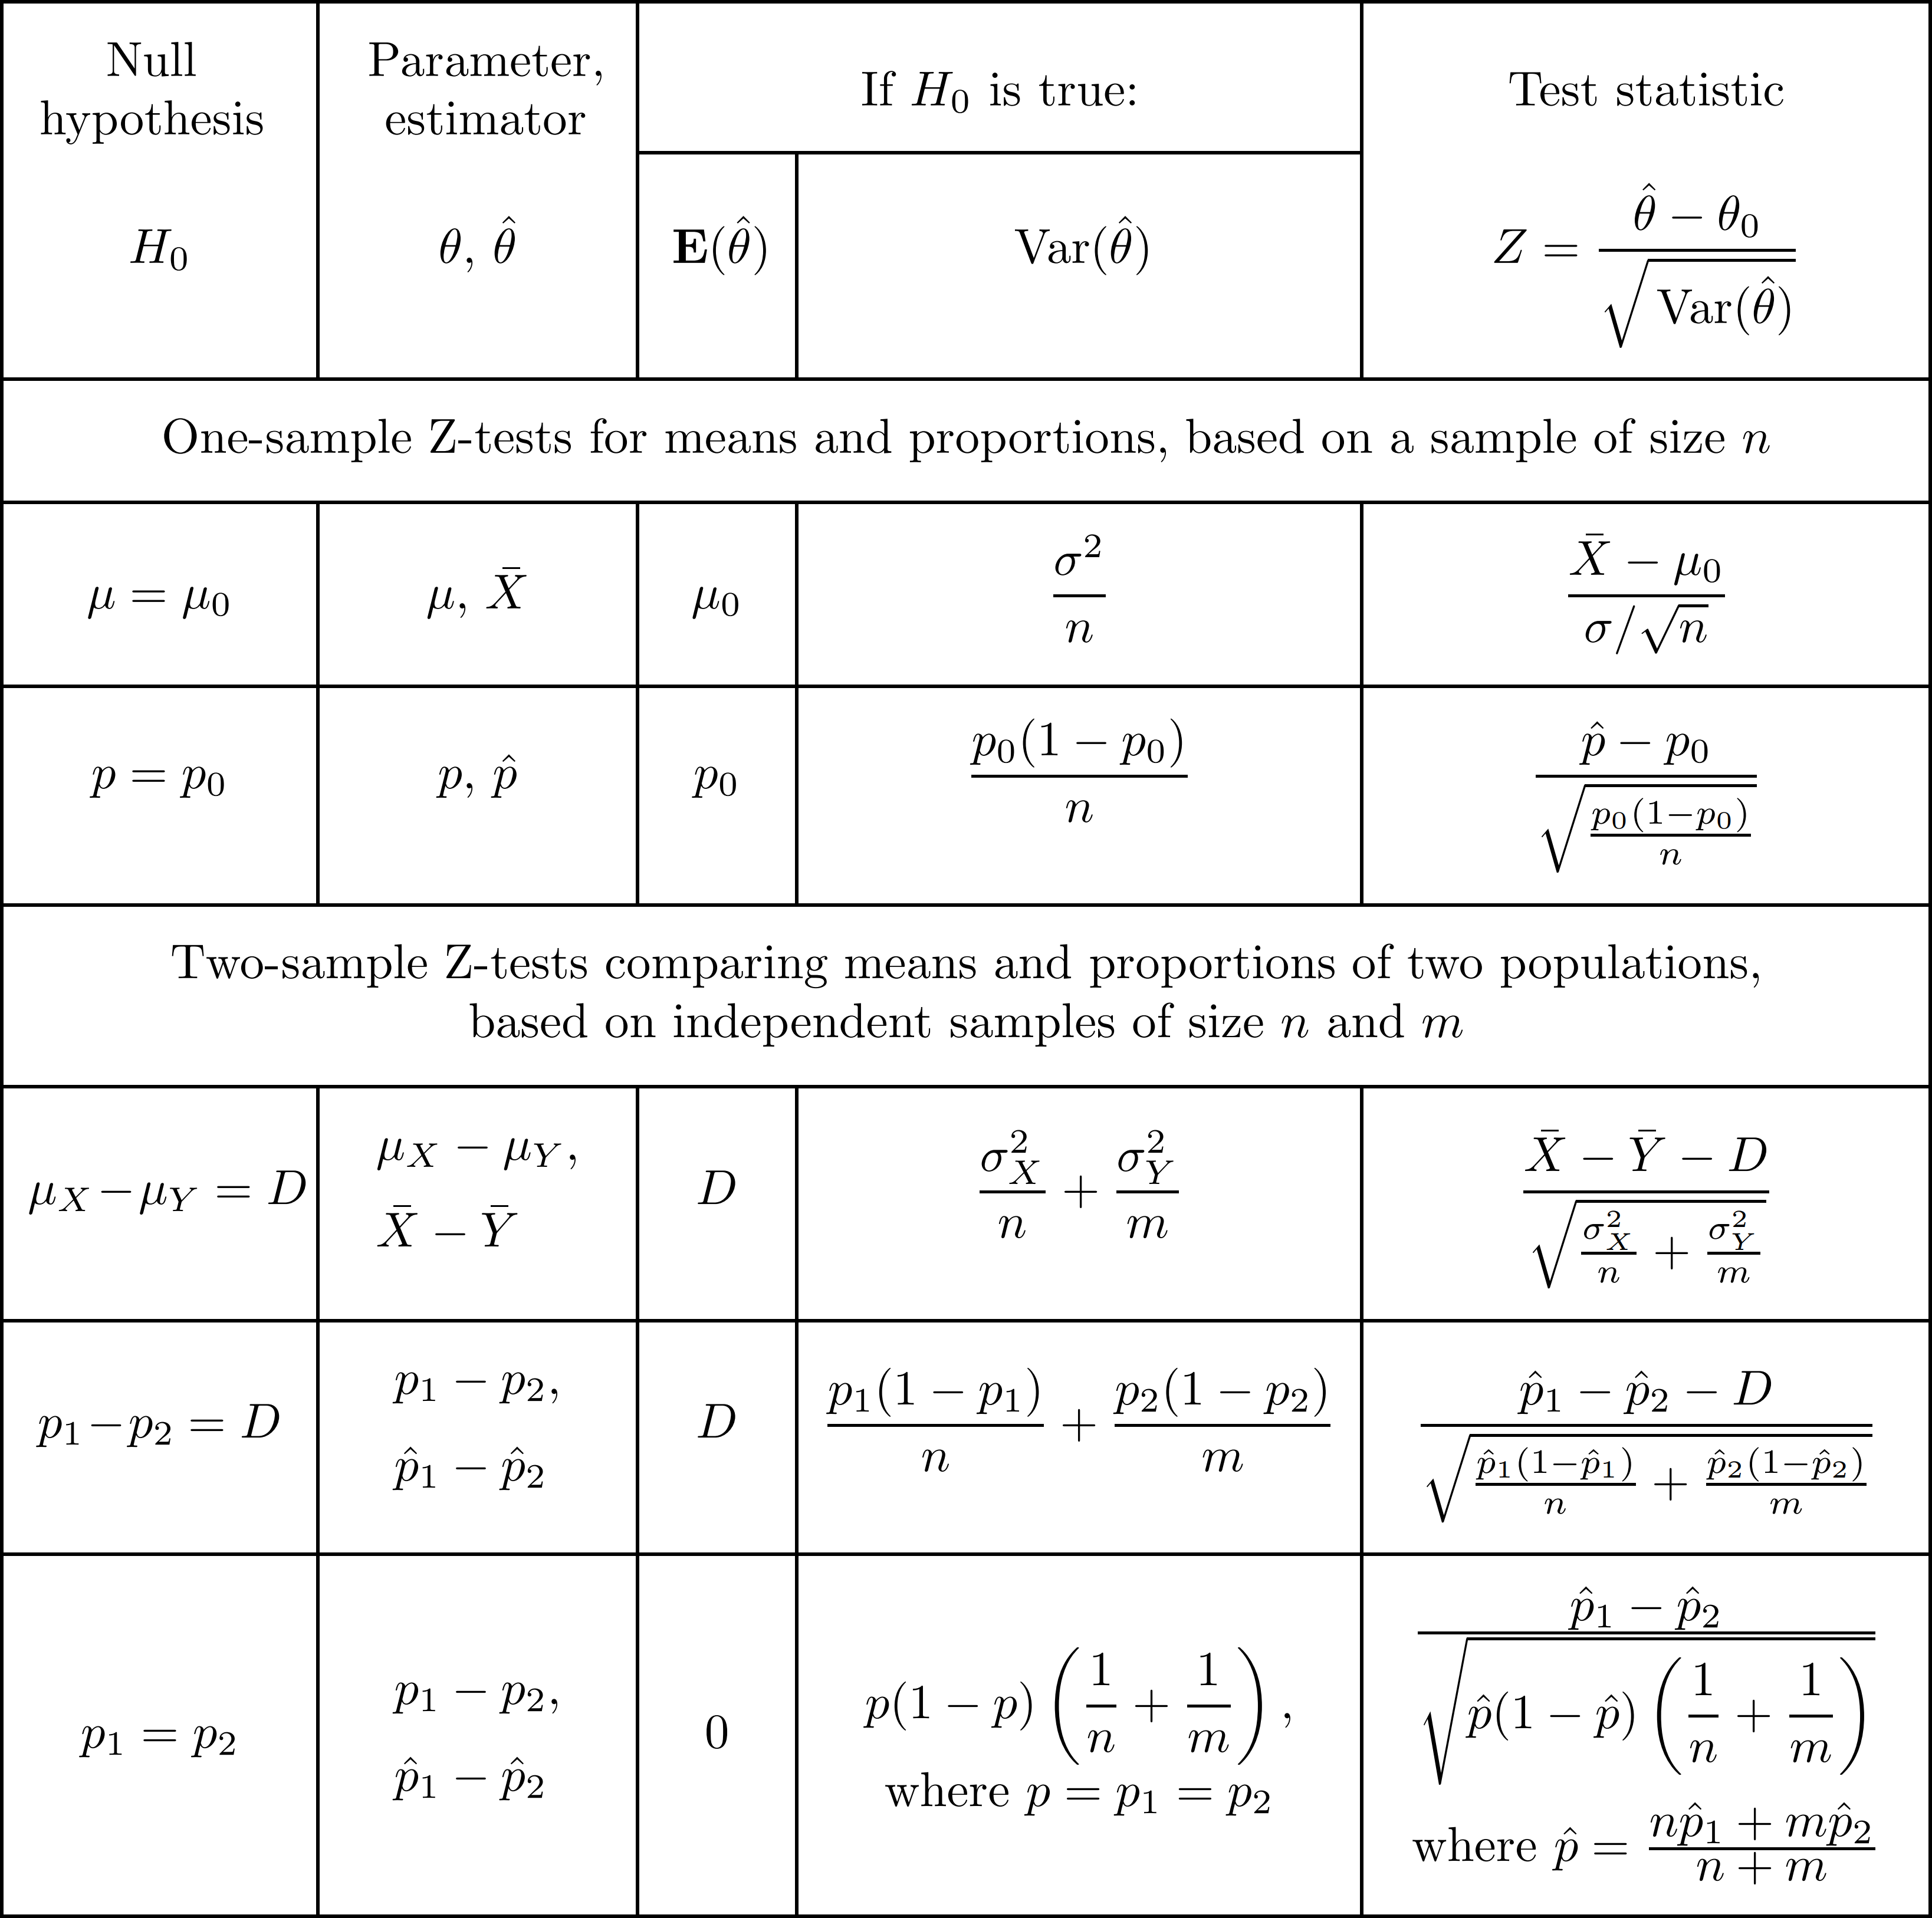
\includegraphics[width=\linewidth]{img/table-9.1.png}
  \caption*{\textbf{Table 1:} \textit{Summary of Z-tests}}
\end{figure}

\newpage

\begin{multicols}{2}
\setlength{\columnsep}{1.5cm}
\setlength{\columnseprule}{0.2pt}

\begin{example}{ (Z-test about a population mean)}
  The number of concurrent users for some internet service provider has always averaged 5000 with a standard deviation of 800. After an equipment upgrade, the average number of users at 100 randomly selected moments of time is 5200. Does it indicate, at a $5\%$ level of significance, that the mean number of concurrent users has increased? Assume that the standard deviation of the number of concurrent users has not changed.

  \textbf{Solution:}
  We test the null hypothesis $H_0\ :\ \mu = 5000$ against a one-sided right-tail alternative $H_A\ :\ \mu > 5000$, because we are only interested to know if the mean number of users $\mu$ has increased.

  \textbf{Step 1:} Test statistic. We are given $\sigma = 800$, $n = 100$, $\alpha = 0.05$, $\mu_0 = 5000$, and from sample, $\bar{X} = 5200$. The test statistic is
  \begin{equation*}
    Z = \frac{\bar{X} - \mu_0}{\sigma / \sqrt{n}} = \frac{5200 - 5000}{800 / \sqrt{100}} = 2.5
  \end{equation*}

  \textbf{Step 2:} Acceptance and rejection regions. The critical value is
  \begin{equation*}
    z_{\alpha} = z_{0.05} = 1.645
  \end{equation*}
  (don't divide $\alpha$ by 2 because it is a one-sided test). With the right-tail alternative, we
  \begin{equation*}
    \begin{cases}
      \textnormal{reject } H_0 &\textnormal{if } Z \geq 1.645\\
      \textnormal{accept } H_0 &\textnormal{if } Z < 1.645\\
    \end{cases}
  \end{equation*}

  \textbf{Step 3:} Result. Our test statistic $Z = 2.5$ belongs to the rejection region; therefore, we reject the null hypothesis. The data (5200 users, on the average, at 100 times) provided sufficient evidence in favor of the alternative hypothesis that the mean number of users has increased.
\end{example}

\begin{example}{ (Two-sample Z-test of proportions)}
  A quality inspector finds 10 defective parts in a sample of 500 parts received from manufacturer A. Out of 400 parts from manufacturer B, she finds 12 defective ones. A computer-making company uses these parts in their computers and claims that the quality of parts produced by A and B is the same. At the $5\%$ level of significance, do we have enough evidence to disprove this claim?

  \textbf{Solution:}
  We test $H_0\ :\ p_A = p_B$, or $H_0\ :\ p_A - p_B = 0$, against $H_A\ :\ p_A \neq p_B$. This is a two-sided test because no direction of the alternative has been indicated. We only need to verify whether or not the proportions of defective parts are equal for manufacturers A and B.

  \textbf{Step 1:} Test statistic. We are given $\\hat{p}_A = 10/500 = 0.02$ from sample size $n = 500$; $\hat{p}_B = 12/400 = 0.03$ from sample size $m = 400$. The tested value is $D = 0$.

  As we know, for these Bernoulli data, the variance depends on the unknown parameters $p_A$ and $p_B$ which are estimated by the sample proportions $\hat{p}_A$ and $\hat{p}_B$.

  The test statistic then equals
  \begin{align*}
    Z &= \dfrac{\hat{p}_A - \hat{p}_B - D}{\sqrt{\dfrac{\hat{p}_A (1 - \hat{p}_A)}{n} + \dfrac{\hat{p}_B (1 - \hat{p}_B)}{m}}} \\
    &= \dfrac{0.02 - 0.03}{\sqrt{\dfrac{(0.02)(0.98)}{500} + \dfrac{(0.03)(0.97)}{400}}} = -0.945
  \end{align*}

  \textbf{Step 2:} Acceptance and rejection regions. This is a two-sided test; thus we divide $\alpha$ by 2, find $z_{0.05/2} = z_{0.025} = 1.96$, and
  \begin{equation*}
    \begin{cases}
      \textnormal{reject } H_0 &\textnormal{if } |Z| \geq 1.96\\
      \textnormal{accept } H_0 &\textnormal{if } |Z| < 1.96\\
    \end{cases}
  \end{equation*}

  \textbf{Step 3:} Result. The evidence against $H_0$ is insufficient because $|Z| < 1.96$. Although sample proportions of defective parts are unequal, the difference between them appears too small to claim that population proportions are different.
\end{example}


\subsection{Pooled Sample Proportion}
\label{subsec:pooled-sample-proportion}

The test in Example 11 can be conducted differently and perhaps, more efficiently. Indeed, we standardize the estimator $\hat{\theta} = \hat{p}_A - \hat{p}_B$ using its expectation $\expc{\hat{\theta}}$ and variance $\var{\hat{\theta}}$ under the null distribution, i.e., when $H_0$ is true. However, under the null hypothesis $p_A = p_B$. Then, when we standardize $(\hat{p}_A - \hat{p}_B)$, instead of estimating two proportions in the denominator, we only need to estimate one.

First, we estimate the common population proportion by the overall proportion of defective parts,
\begin{align*}
  \hat{p}(\textnormal{pooled}) &= \frac{\textnormal{number of defective parts}}{\textnormal{total number of parts}} \\
  &= \frac{n\hat{p}_A + m\hat{p}_B}{n + m}
\end{align*}
Then we estimate the common variance as
\begin{align*}
  \widehat{\textnormal{Var}}(\hat{p}_A - \hat{p}_B) &= \frac{\hat{p} (1 - \hat{p})}{n} + \frac{\hat{p} (1 - \hat{p})}{m} \\
  &= \hat{p}(1 - \hat{p}_A) \left( \frac{1}{n} + \frac{1}{m} \right)
\end{align*}
and use it for the Z-statistic,
\begin{align*}\
  Z = \dfrac{\hat{p}_A - \hat{p}_B}{\sqrt{\hat{p} (1 - \hat{p}) \left( \dfrac{1}{n} + \dfrac{1}{m} \right)}}
\end{align*}

\begin{example}{ (Example 11, continued)}
  Here the pooled proportion equals
  \begin{equation*}
    \hat{p} = \frac{10 + 12}{500 + 400} = 0.0244
  \end{equation*}
  so that
  \begin{equation*}
    Z = \frac{0.02 - 0.03}{\sqrt{(0.0244)(0.9756) \left( \frac{1}{500} + \frac{1}{400} \right)}} = -0.966
  \end{equation*}
  This does not affect our result. We obtained a different value of Z-statistic, but it also belongs to the acceptance region. We still don't have a significant evidence against the equality of two population proportions.
\end{example}
  

\subsection{Unknown \texorpdfstring{$\sigma$}{sigma}: T-tests}
\label{subsec:T-test}

As we decided in Section 3, when we don't know the population standard deviation, we estimate it. The resulting T-statistic has the form
\begin{align*}
  t =   \frac{\hat{\theta} - \expc{\hat{\theta}}}{s(\hat{\theta})} = \frac{\hat{\theta} - \expc{\hat{\theta}}}{\sqrt{\widehat{\textnormal{Var}(\hat{\theta})}}}
\end{align*}
In the case when the distribution of $\hat{\theta}$ is Normal, the test is based on Student's T-distribution with acceptance and rejection regions according to the direction of $H_A$:
\begin{enumerate}[label=(\alph*)]
  \item For a \textbf{right-tail alternative},
    \begin{equation}
      \begin{cases}
        \textnormal{reject } H_0 &\textnormal{if } t \geq t_{\alpha}\\
        \textnormal{accepts } H_0 &\textnormal{if } t < t_{\alpha}\\
      \end{cases}
    \end{equation}
  
  \item For a \textbf{left-tail alternative},
    \begin{equation}
      \begin{cases}
        \textnormal{reject } H_0 &\textnormal{if } t \leq -t_{\alpha}\\
        \textnormal{accepts } H_0 &\textnormal{if } t > -t_{\alpha}\\
      \end{cases}      
    \end{equation}
  
  \item For a \textbf{two-sided alternative},
    \begin{equation}
      \begin{cases}
        \textnormal{reject } H_0 &\textnormal{if } |t| \geq t_{\alpha/2}\\
        \textnormal{accepts } H_0 &\textnormal{if } |t| < t_{\alpha/2}\\
      \end{cases}
    \end{equation}
\end{enumerate}
Quantiles $t_{\alpha}$ and $t_{\alpha/2}$ are given in Table A5 (in textbook). As in Section 3.4, the number of degrees of freedom depends on the problem and the sample size, see Table 2 and formula (10)
\end{multicols}

\begin{figure}[H]
  \centering
  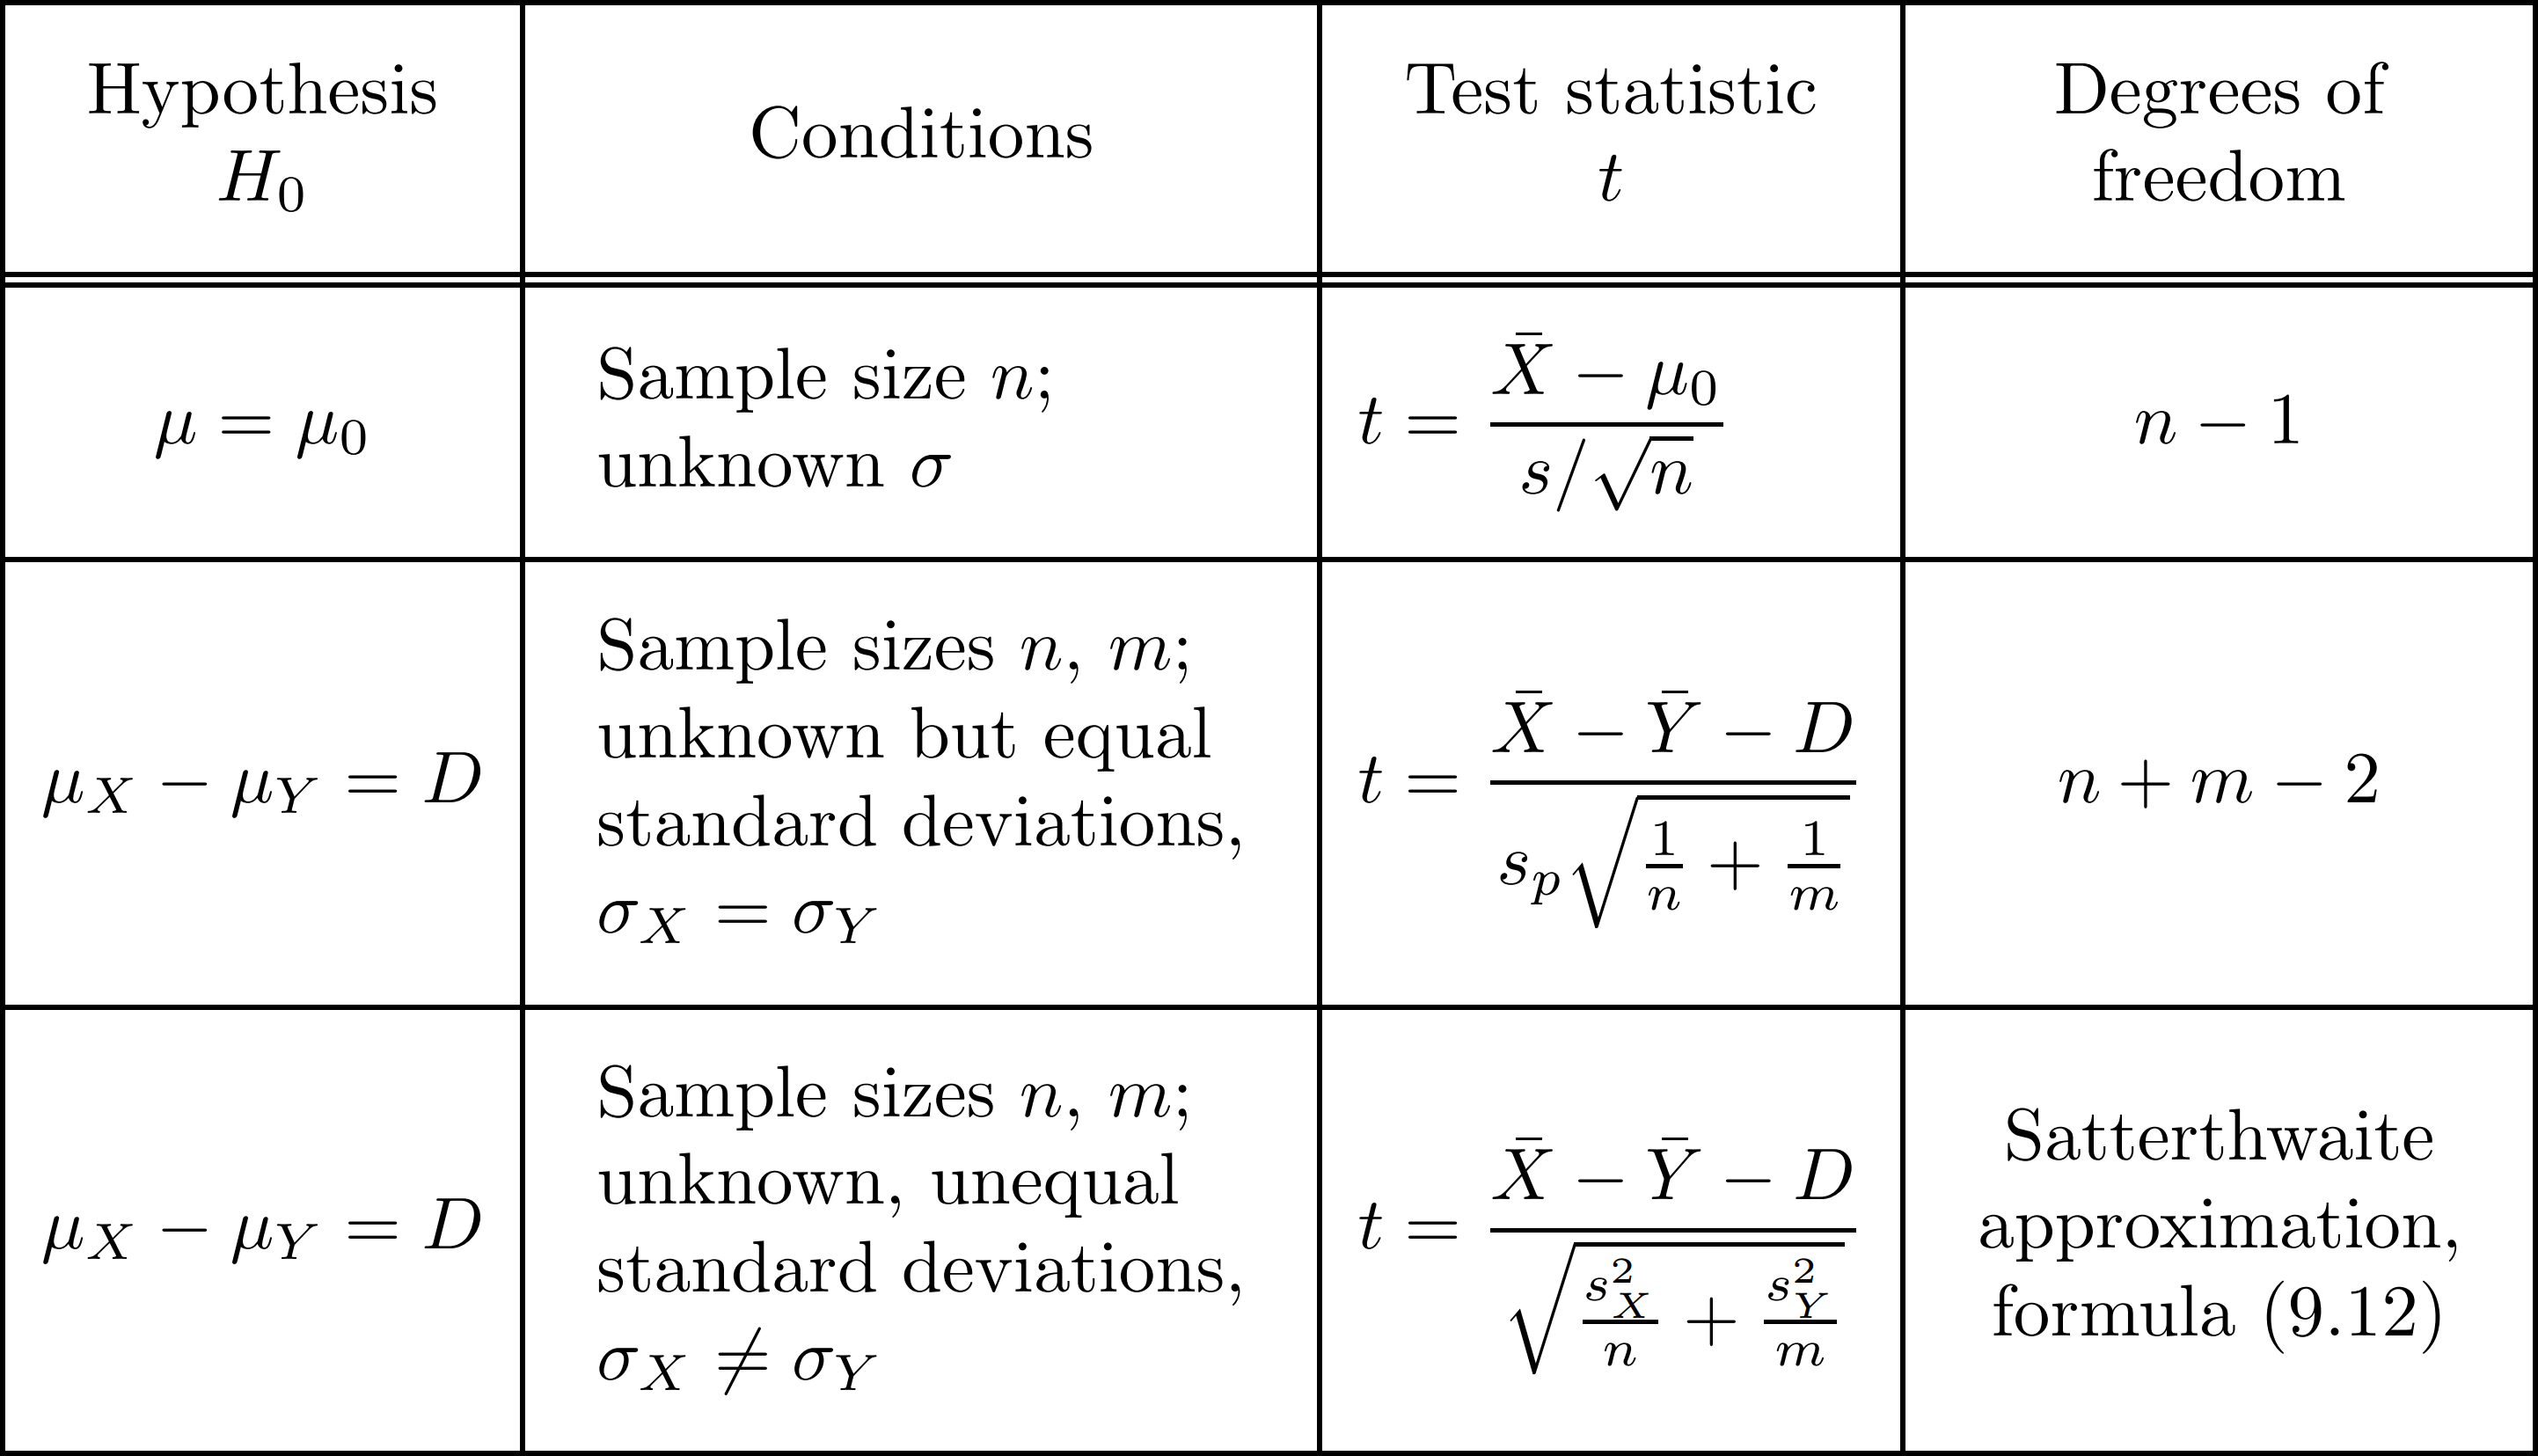
\includegraphics[width=\linewidth]{img/table-9.2.png}
  \caption*{\textbf{Table 2:} \textit{Summary of T-tests}}
  \label{table2}
\end{figure}

\begin{multicols}{2}
\setlength{\columnsep}{1.5cm}
\setlength{\columnseprule}{0.2pt}

As in Section 3.4, the \textbf{pooled sample variance}
\begin{align*}
  s_p^2 &= \frac{\dsum_{i = 1}^{n} (X_i - \bar{X})^2 + \dsum_{i = 1}^{m} (Y_i - \bar{Y})^2}{n + m - 2} \\
  &= \frac{(n - 1) s_X^2 + (m - 1) s_Y^2}{n + m - 2}
\end{align*}
is computed for the case of equal unknown variances. When variances are not equal, degrees of freedom are computed by Satterthwaite approximation (12).

\textbf{\textit{Check examples 9.28, 9.29, 9.30 in the textbook}}.

When the distribution of $\hat{\theta}$ is not Normal, the Student's \textit{T-distribution} cannot be used. The distribution of a T-statistic and all its probabilities will be different from Student's T, and as a result, our test may not have the desired significance level.


\subsection{Duality: Two-sided Tests and Two-sided Confidence Intervals}
\label{subsec:duality}

An interesting fact can be discovered if we look into our derivation of tests and confidence intervals. It turns out that we can conduct two-sided tests using nothing but the confidence intervals!
\begin{formula}{(Eq. 21)}
  A level $\alpha$ Z-test of $H_0\ :\ \theta = \theta_0$ vs $H_A\ :\ \theta \neq \theta_0$ accepts the null hypothesis 
  
  \begin{center}\textit{\textbf{if and only if}}\end{center}

  a symmetric $(1 - \alpha)100\%$ confidence Z-interval for $\theta$ contains $\theta_0$.
\end{formula}
\setcounter{equation}{21}

\begin{figure}[H]
  \centering
  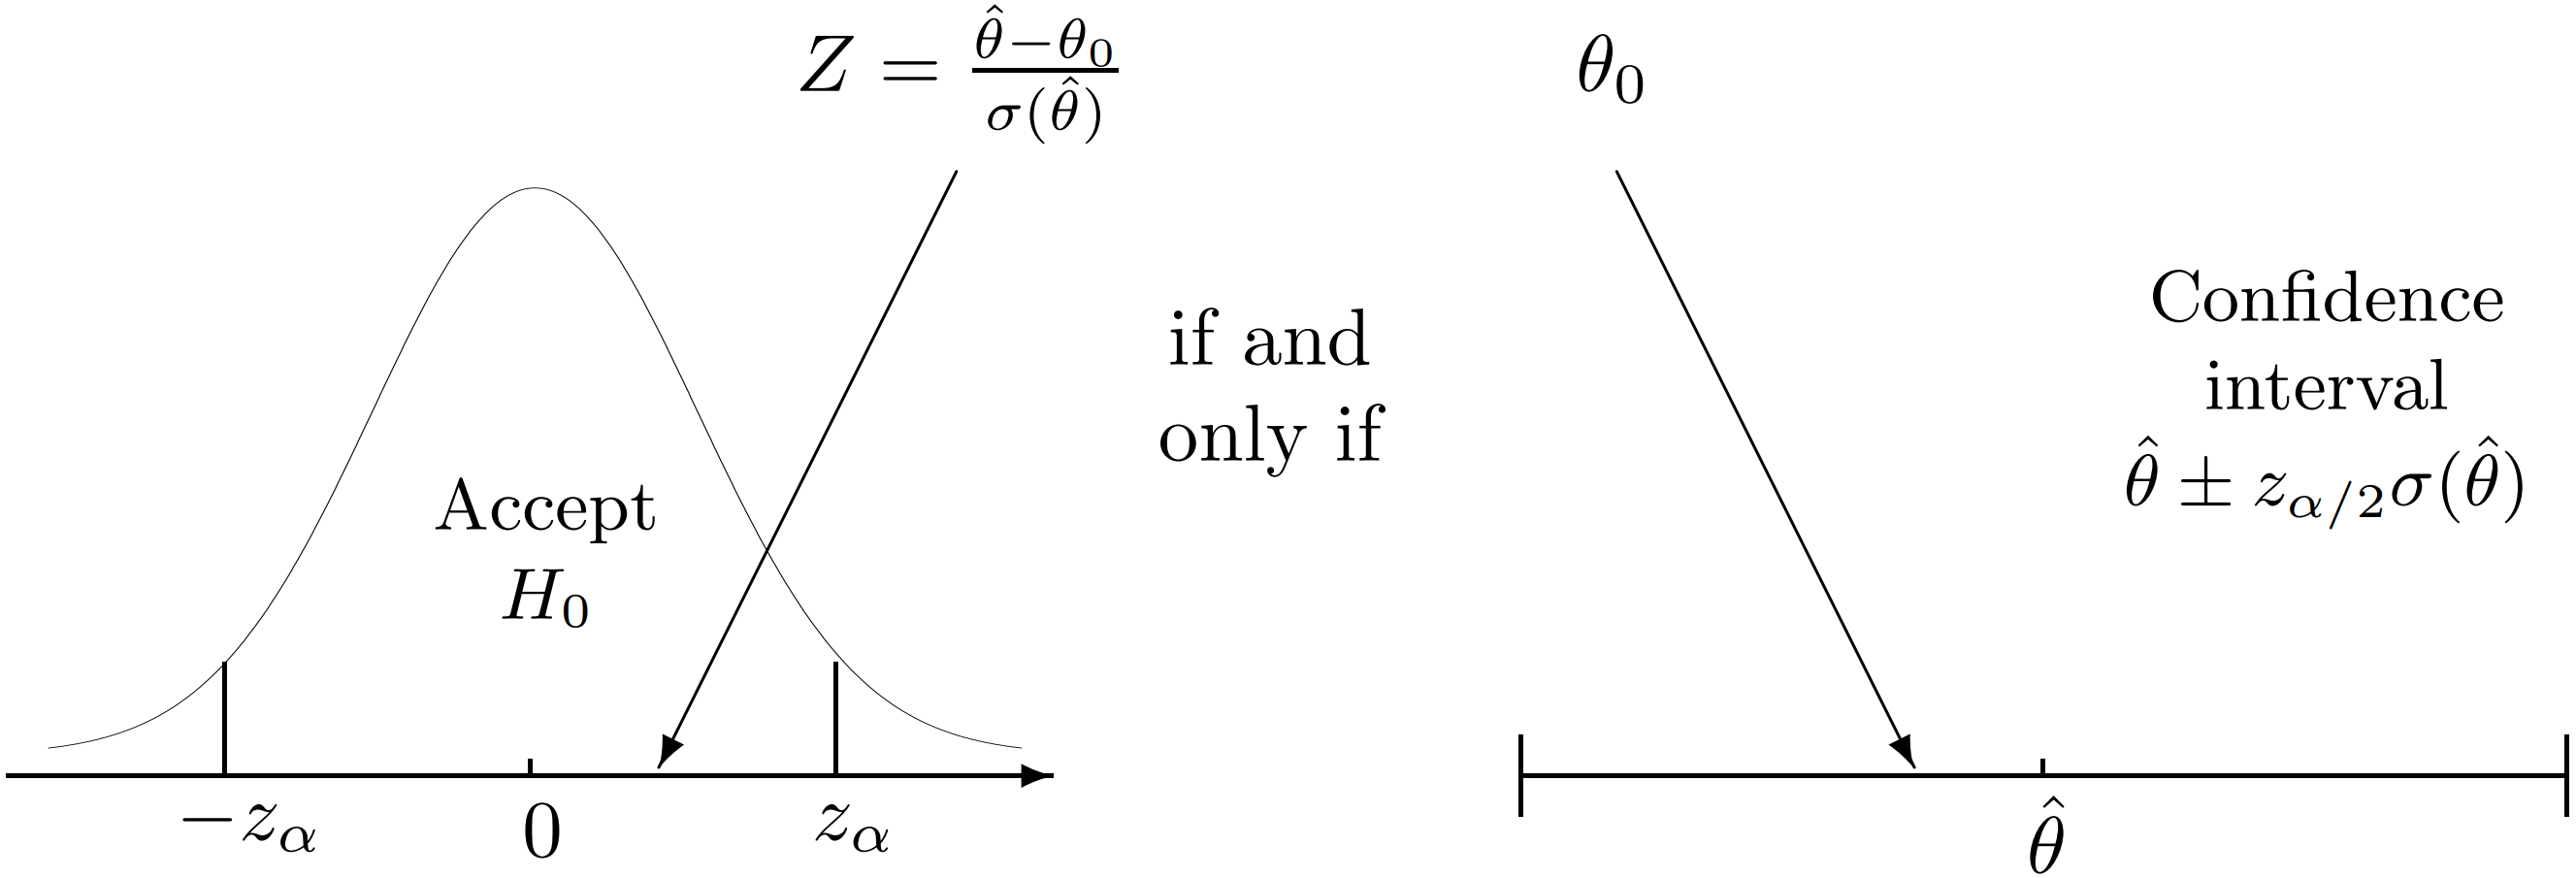
\includegraphics[width=\linewidth]{img/fig-9.8.png}
  \caption{}
\end{figure}

In fact, any two-sided test can be conducted this way. Accept $H_0\ :\ \theta = \theta_0$ whenever a $(1 - \alpha)100\%$ confidence interval for $\theta$ covers $\theta_0$. Under $\theta_0$, this test will accept the null
hypothesis as often as the interval will cover $\theta_0$, i.e., with probability $(1 - \alpha)$. Thus, we have a level $\alpha$ test.

Rule (21) applies only when
\begin{itemize}
  \item we are testing against a two-sided alternative (notice that our confidence intervals are two-sided too);
  \item significance level $\alpha$ of the test matches confidence level $(1 - \alpha)$ of the confidence interval. For example, a two-sided $3\%$ level test can be conducted using a $97\%$ confidence interval.
\end{itemize}

\begin{example}{}
  A sample of 6 measurements
  \begin{center}
    2.5, 7.4, 8.0, 4.5, 7.4, 9.2
  \end{center}
  is collected from a Normal distribution with mean $\mu$ and standard deviation $\sigma = 2.2$. Test whether $\mu = 6$ against a two-sided alternative $H_A\ :\ \mu \neq 6$ at the $5\%$ level of significance.

  \textbf{Solution:}
  Solving Example 4, we have already constructed a $95\%$ confidence interval for $\mu$,
  \begin{equation*}
    \left[ 4.74,\ 8.26 \right]
  \end{equation*}
  The value of $\mu_0 = 6$ belongs to it; therefore, at the $5\%$ level, the null hypothesis is accepted.
\end{example}

\begin{example}{}
  Use data in Example 13 to test whether $\mu = 7$.

  \textbf{Solution:}
  The interval $\left[ 4.74,\ 8.26 \right]$ contains $\mu_0 = 7$ too; therefore, the hypothesis $H_0\ :\ \mu = 7$ is accepted as well.
\end{example}

\textbf{\textit{Check examples 9.33, 9.34, 9.35 in the textbook}}.

Similarly, for the case of unknown variance(s).
\begin{formula}{}
  A level $\alpha$ T-test of $H_0\ :\ \theta = \theta_0$ vs $H_A\ :\ \theta \neq \theta_0$ accepts the null hypothesis 
  
  \begin{center}\textit{\textbf{if and only if}}\end{center}

  a symmetric $(1 - \alpha)100\%$ confidence T-interval for $\theta$ contains $\theta_0$.
\end{formula}



\end{multicols}

\end{document}
